\documentclass[3p]{elsarticle}

\biboptions{super,sort&compress}

% Standard package includes for math, tables, and images
\usepackage{float}
\usepackage{enumitem}
\usepackage{subcaption}
\usepackage{amsmath}
\usepackage{booktabs}
\usepackage{graphicx}
\usepackage{url}
\usepackage{stfloats}
\usepackage{tabularx}
\usepackage{setspace}
\usepackage{xcolor}

% Font and layout improvements
\usepackage[T1]{fontenc}
\usepackage[utf8]{inputenc}
\usepackage{microtype}
\usepackage{inconsolata}
\usepackage{hyperref}

% Visible author placeholders -- remove all before submission
\newcommand{\authortodo}[1]{\textcolor{red}{\textbf{[TODO: #1]}}}

\journal{Digital Discovery (manuscript prepared for submission)}

\emergencystretch=3em
\begin{document}

\begin{frontmatter}

    \title{Perovskite Solar Cell Performance Prediction with LLM-Derived Feature Augmentation under Leakage-Aware DOI Evaluation}

    \author[1]{Sunraj Patel}
    \author[1]{Shikhar Misra\corref{cor1}}

    \cortext[cor1]{Corresponding author.}
    \ead{shikharm@iitk.ac.in}

    \address[1]{Department of Materials Science and Engineering, Indian Institute of Technology Kanpur, India 208016}


    \begin{abstract}
        Machine-learning (ML) models for perovskite solar cell (PSC) performance are increasingly trained on literature-derived databases such as the Perovskite Database Project (PDP), yet the PDP studies that describe their partitioning use record-level splits, even though a single publication often contributes many closely related device records. Here we build a power conversion efficiency (PCE) prediction framework on 41,107 PDP device records from 7,326 publications, combining device and fabrication variables and composition descriptors ($t_1$), curated material properties ($t_2$) and publication-level features extracted from full texts with a locally served large language model (LLM, $t_3^{\mathrm{orig}}$). Models are evaluated with repeated DOI-grouped holdouts that use a DOI-disjoint validation set for early stopping, so that no test publication influences training or model selection. With one fixed CatBoost configuration, the pooled $R^2$ on unseen publications is $0.368 \pm 0.024$, $0.408 \pm 0.032$ and $0.407 \pm 0.031$ for $t_1$, $t_2$ and the original literature block (MAE 2.96 percentage points; mean $\pm$ s.d. over five overlapping holdouts); a validation-tuned CatBoost--XGBoost ensemble reaches $0.418 \pm 0.026$ (MAE 2.92). Material-property descriptors give a measurable gain ($\Delta R^2 = +0.040$, paired DOI-cluster bootstrap interval excluding zero in all five pooled splits), but a material-identity control recovers essentially all of it, so the gain reflects knowing which materials are present; the original literature block gives no detectable gain ($\Delta R^2 = -0.001$ pooled). Our final LLM-derived representation is a block of 36 binary recipe flags (additive and precursor identities, electron- and hole-transport-layer dopants, process route and device context) built from the stored extraction output, available for 36.6\% of records. Scored once on reserved publications, adding the flags to $t_2$ changed $R^2$ by $+0.0071$ (95\% interval $-0.0007$ to $+0.0157$) on publications with extraction data and by $+0.0025$ ($-0.0011$ to $+0.0062$) on all records under the same default settings, and by $+0.0094$ ($-0.0016$ to $+0.0219$; $R^2$ 0.361 to 0.371) and $+0.0015$ ($-0.0039$ to $+0.0067$) when each tier used its own tuned settings. All intervals include zero, so we describe these as small, suggestive improvements that are not statistically established. Under matched features and budgets, record-level random splitting yields a converged CatBoost $R^2$ of 0.59--0.63, i.e.\ 0.21--0.22 higher than DOI-grouped evaluation, while a ridge model shows a gap of only 0.06; 69\% of PCE variance lies between publications. DOI-grouped evaluation therefore gives a more defensible estimate of performance on new publications, while lead-author grouping changes little (0.395) and forward-in-time evaluation lowers it to 0.335; no external validation was possible.
    \end{abstract}

    \begin{keyword}
        Perovskite solar cells; Power conversion efficiency; Materials informatics; Large language models; Data leakage; SHAP interpretability.
    \end{keyword}

\end{frontmatter}

% ---------------- INTRODUCTION ----------------
\section{Introduction}

Perovskite solar cells (PSCs) are promising photovoltaic devices whose performance depends on the absorber material, device architecture, and fabrication conditions. A typical planar PSC consists of five functional layers: a substrate, an electron transport layer (ETL), a perovskite absorber, a hole transport layer (HTL), and a metal electrode. As illustrated in Fig.~\ref{fig:psc_structures}, two widely used configurations are n-i-p and p-i-n, which differ in the relative positions of the ETL and HTL \cite{jung2015perovskite,zuo2016advances}. Under illumination, the perovskite absorber generates charge carriers, while the ETL and HTL selectively transport electrons and holes, respectively, towards the electrodes. Charge extraction and recombination, together with the properties of the constituent materials, influence the resulting photovoltaic performance \cite{jung2015perovskite,zuo2016advances}.

Power conversion efficiency (PCE) is the principal metric of PSC performance and represents the fraction of incident optical power converted into electrical power. The fill factor (FF) characterizes the shape of the current--voltage curve as the ratio of the maximum output power to the product of the open-circuit voltage and short-circuit current. These quantities are expressed as
\begin{equation}
    \mathrm{PCE} =
    \frac{V_{\mathrm{OC}}J_{\mathrm{SC}}\mathrm{FF}}{P_{\mathrm{in}}}
    \times 100\%,
\end{equation}
and
\begin{equation}
    \mathrm{FF} =
    \frac{V_{\mathrm{MPP}}J_{\mathrm{MPP}}}
    {V_{\mathrm{OC}}J_{\mathrm{SC}}},
\end{equation}
where $V_{\mathrm{OC}}$ and $J_{\mathrm{SC}}$ denote the open-circuit voltage and short-circuit current density, respectively; $V_{\mathrm{MPP}}$ and $J_{\mathrm{MPP}}$ are the voltage and current density at the maximum power point; and $P_{\mathrm{in}}$ is the incident optical power density \cite{zuo2016advances}. The dependence of PCE on multiple interacting material, architectural, and processing variables makes systematic device optimization challenging. Machine learning (ML) offers a data-driven approach to identifying these relationships and exploring combinations of experimentally reported parameters that would be difficult to investigate exhaustively through conventional trial-and-error approaches \cite{odabasi2019performance,bansal2023machine,li2019predictions,liu2022machine,gok2022predicting}.

\begin{figure}[t]
    \centering
    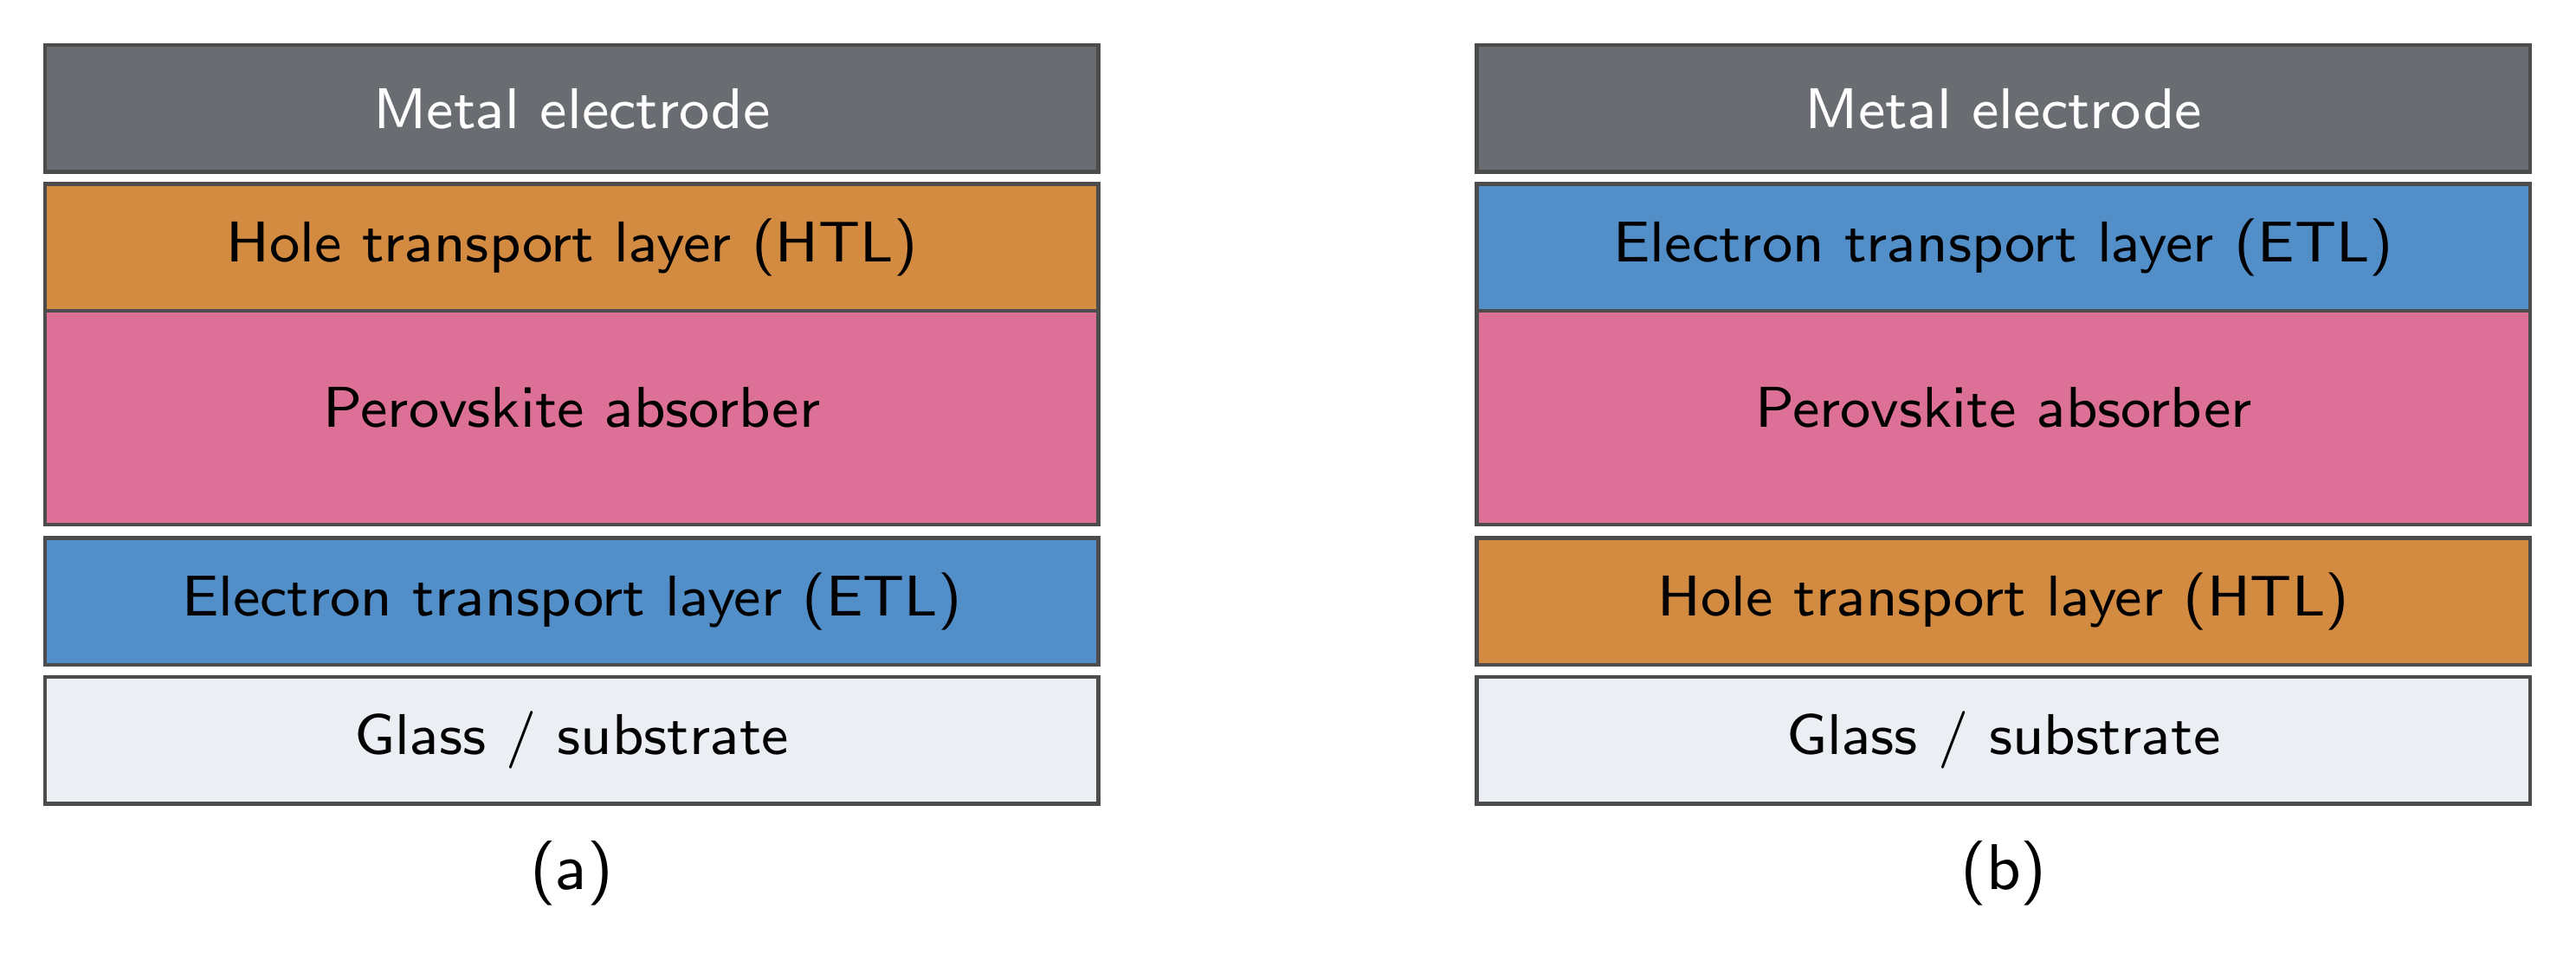
\includegraphics[width=0.95\textwidth]{figures/device_structure.png}
    \caption{Example device structure for a (a) n-i-p and (b) p-i-n perovskite solar cell.}
    \label{fig:psc_structures}
\end{figure}

The availability of large experimental databases has enabled ML models to be developed using combinations of material, device, and process information. The Perovskite Database Project (PDP) provides an open-access collection of PSC data covering material compositions, device structures, fabrication conditions, and photovoltaic characteristics \cite{jacobsson2022open}. Roberts et al. developed an open-source ML pipeline using the PDP and evaluated XGBoost, artificial neural networks, and Gaussian process regression for predicting short-circuit current density. Their XGBoost model achieved a test $R^2$ of 0.35 and an RMSE of $3.58$ mA cm$^{-2}$, while their analysis highlighted the importance of data cleaning, feature encoding, and reproducible workflows \cite{roberts2024machine}. Other device-level studies have similarly examined the influence of descriptor selection and dataset characteristics on predictive performance \cite{sala2023assessing}.

Fukasawa et al. examined the representation of material and process information specifically for PCE prediction using the PDP \cite{fukasawa2024effectiveness}. Starting with 42,459 records, they curated the dataset to obtain 36,937 records with 248 material- and process-related variables. Their results demonstrated that incorporating process information improved prediction compared with using perovskite composition alone. Under an 8:2 train--test split (the article does not describe grouping by publication), their best feature representation achieved a test $R^2$ of 0.7177; however, evaluation on 294 newly registered records yielded an $R^2$ of 0.45 and an MAE of 3.20\% \cite{fukasawa2024effectiveness}. They also identified substantial data degeneracy, with 6,446 unique degenerate points corresponding to 20,695 feature vectors, indicating that distinct experimental records can have identical feature representations despite exhibiting different PCE values.

The distinction between interpolation within an existing dataset and generalization to new groups of observations is also recognized in the broader materials-informatics and machine-learning literature. Meredig et al. introduced leave-one-cluster-out cross-validation to examine how evaluation strategies affect estimates of model performance for materials discovery, emphasizing that conventional random validation may not adequately represent extrapolative use cases \cite{meredig2018cluster}. More broadly, Kapoor and Narayanan documented data leakage as a recurring source of overoptimistic findings and reproducibility problems across scientific machine-learning applications \cite{kapoor2023leakage}. These studies establish that evaluation should reflect the intended generalization setting and the dependence structure of the data. In literature-compiled PSC datasets, publication DOI provides a practical grouping variable for assessing performance on papers excluded from training. Our work applies this principle to PCE prediction and quantifies how the estimated performance and feature-tier comparisons change when publication-level overlap is removed.

The literature-derived nature of PSC databases raises a further concern about model evaluation. Multiple devices reported in the same publication may share material selections, fabrication procedures, device architectures, and measurement conditions, making record-level independence an assumption that requires scrutiny. Roberts et al.\ released an open-source cleaning and modelling pipeline for the Perovskite Database Project (PDP) with short-circuit current density as the target; repeated device configurations that arose during their feature reduction were replaced by a single pseudo-target, and the models were evaluated on an 80/10/10 train/validation/test split \cite{roberts2024machine}. Fukasawa et al. reported a reduction in predictive performance from \(R^2=0.7177\) under their conventional evaluation to \(R^2=0.45\) with an MAE of \(3.20\) percentage points on 294 newly registered records \cite{fukasawa2024effectiveness}. This result provides prior evidence that performance estimates can be sensitive to the evaluation set and the distribution of newly reported devices. However, the newly registered-record evaluation was relatively small and was not presented as a systematic DOI-grouped cross-validation protocol. Of the PDP-based studies we examined, the two that describe their partitioning use record-level splits \cite{roberts2024machine,fukasawa2024effectiveness}, and a further PCE study does not state its splitting procedure \cite{hussain2023leveraging}. Group-aware, cluster-based, forward and time-split validation are established in materials informatics, cheminformatics and ecology \cite{meredig2018cluster,stanev2018superconductor,kauwe2020extraordinary,xiong2020forward,sheridan2013timesplit,roberts2017crossvalidation}; the contribution here is narrower. To our knowledge, no earlier study compares record-level and DOI-grouped evaluation on the same PDP export under matched features, preprocessing and model settings (our literature search was not exhaustive), and we do so here. Such evaluation prevents records sharing a DOI from appearing in both training and test partitions, providing a direct assessment of generalization to publications excluded from training.


In this work, we develop a literature- and material-augmented ML framework for predicting PSC PCE from the PDP, and evaluate it at the publication level. The contributions are twofold.
\begin{enumerate}[label=(\roman*)]
    \item \textbf{Controlled feature ablation and an LLM-derived recipe block.} We combine PDP device and fabrication variables with composition-derived descriptors, curated layer-resolved material properties, and publication-level features extracted from the full text of 2,699 matched articles using a locally served LLM. Nested feature tiers are compared with one fixed CatBoost configuration, identical splits and validation-based early stopping. Material-property descriptors give a measurable gain on unseen publications, which a material-identity control attributes to knowing which materials are used; an original block of 44 literature predictors adds no measurable gain over the material tier. We then construct a final LLM-derived representation, 36 binary recipe flags covering additive and precursor identities, transport-layer dopants, process route and device context, and score it once on reserved publications: the point estimates favour the flags (about $+0.007$ $R^2$ on publications with extraction data under matched settings), but all intervals include zero and coverage is limited to 36.6\% of records.
    \item \textbf{Publication-level evaluation.} We compare record-level random splitting with repeated DOI-grouped holdouts under matched feature tiers, models, preprocessing and budgets, with DOI normalisation, an explicit treatment of records lacking a DOI, and a DOI-disjoint validation set so that no model selection touches the test publications. We quantify the gap for a flexible (CatBoost) and a linear (ridge) model and relate it to the within-publication structure of the data.
\end{enumerate}

SHAP-based interpretation is further used to characterize the features associated with model predictions in the n-i-p and p-i-n architectures. The overall workflow is summarized in Fig.~\ref{fig:ml_workflow}.

\begin{figure}[t]
    \centering
    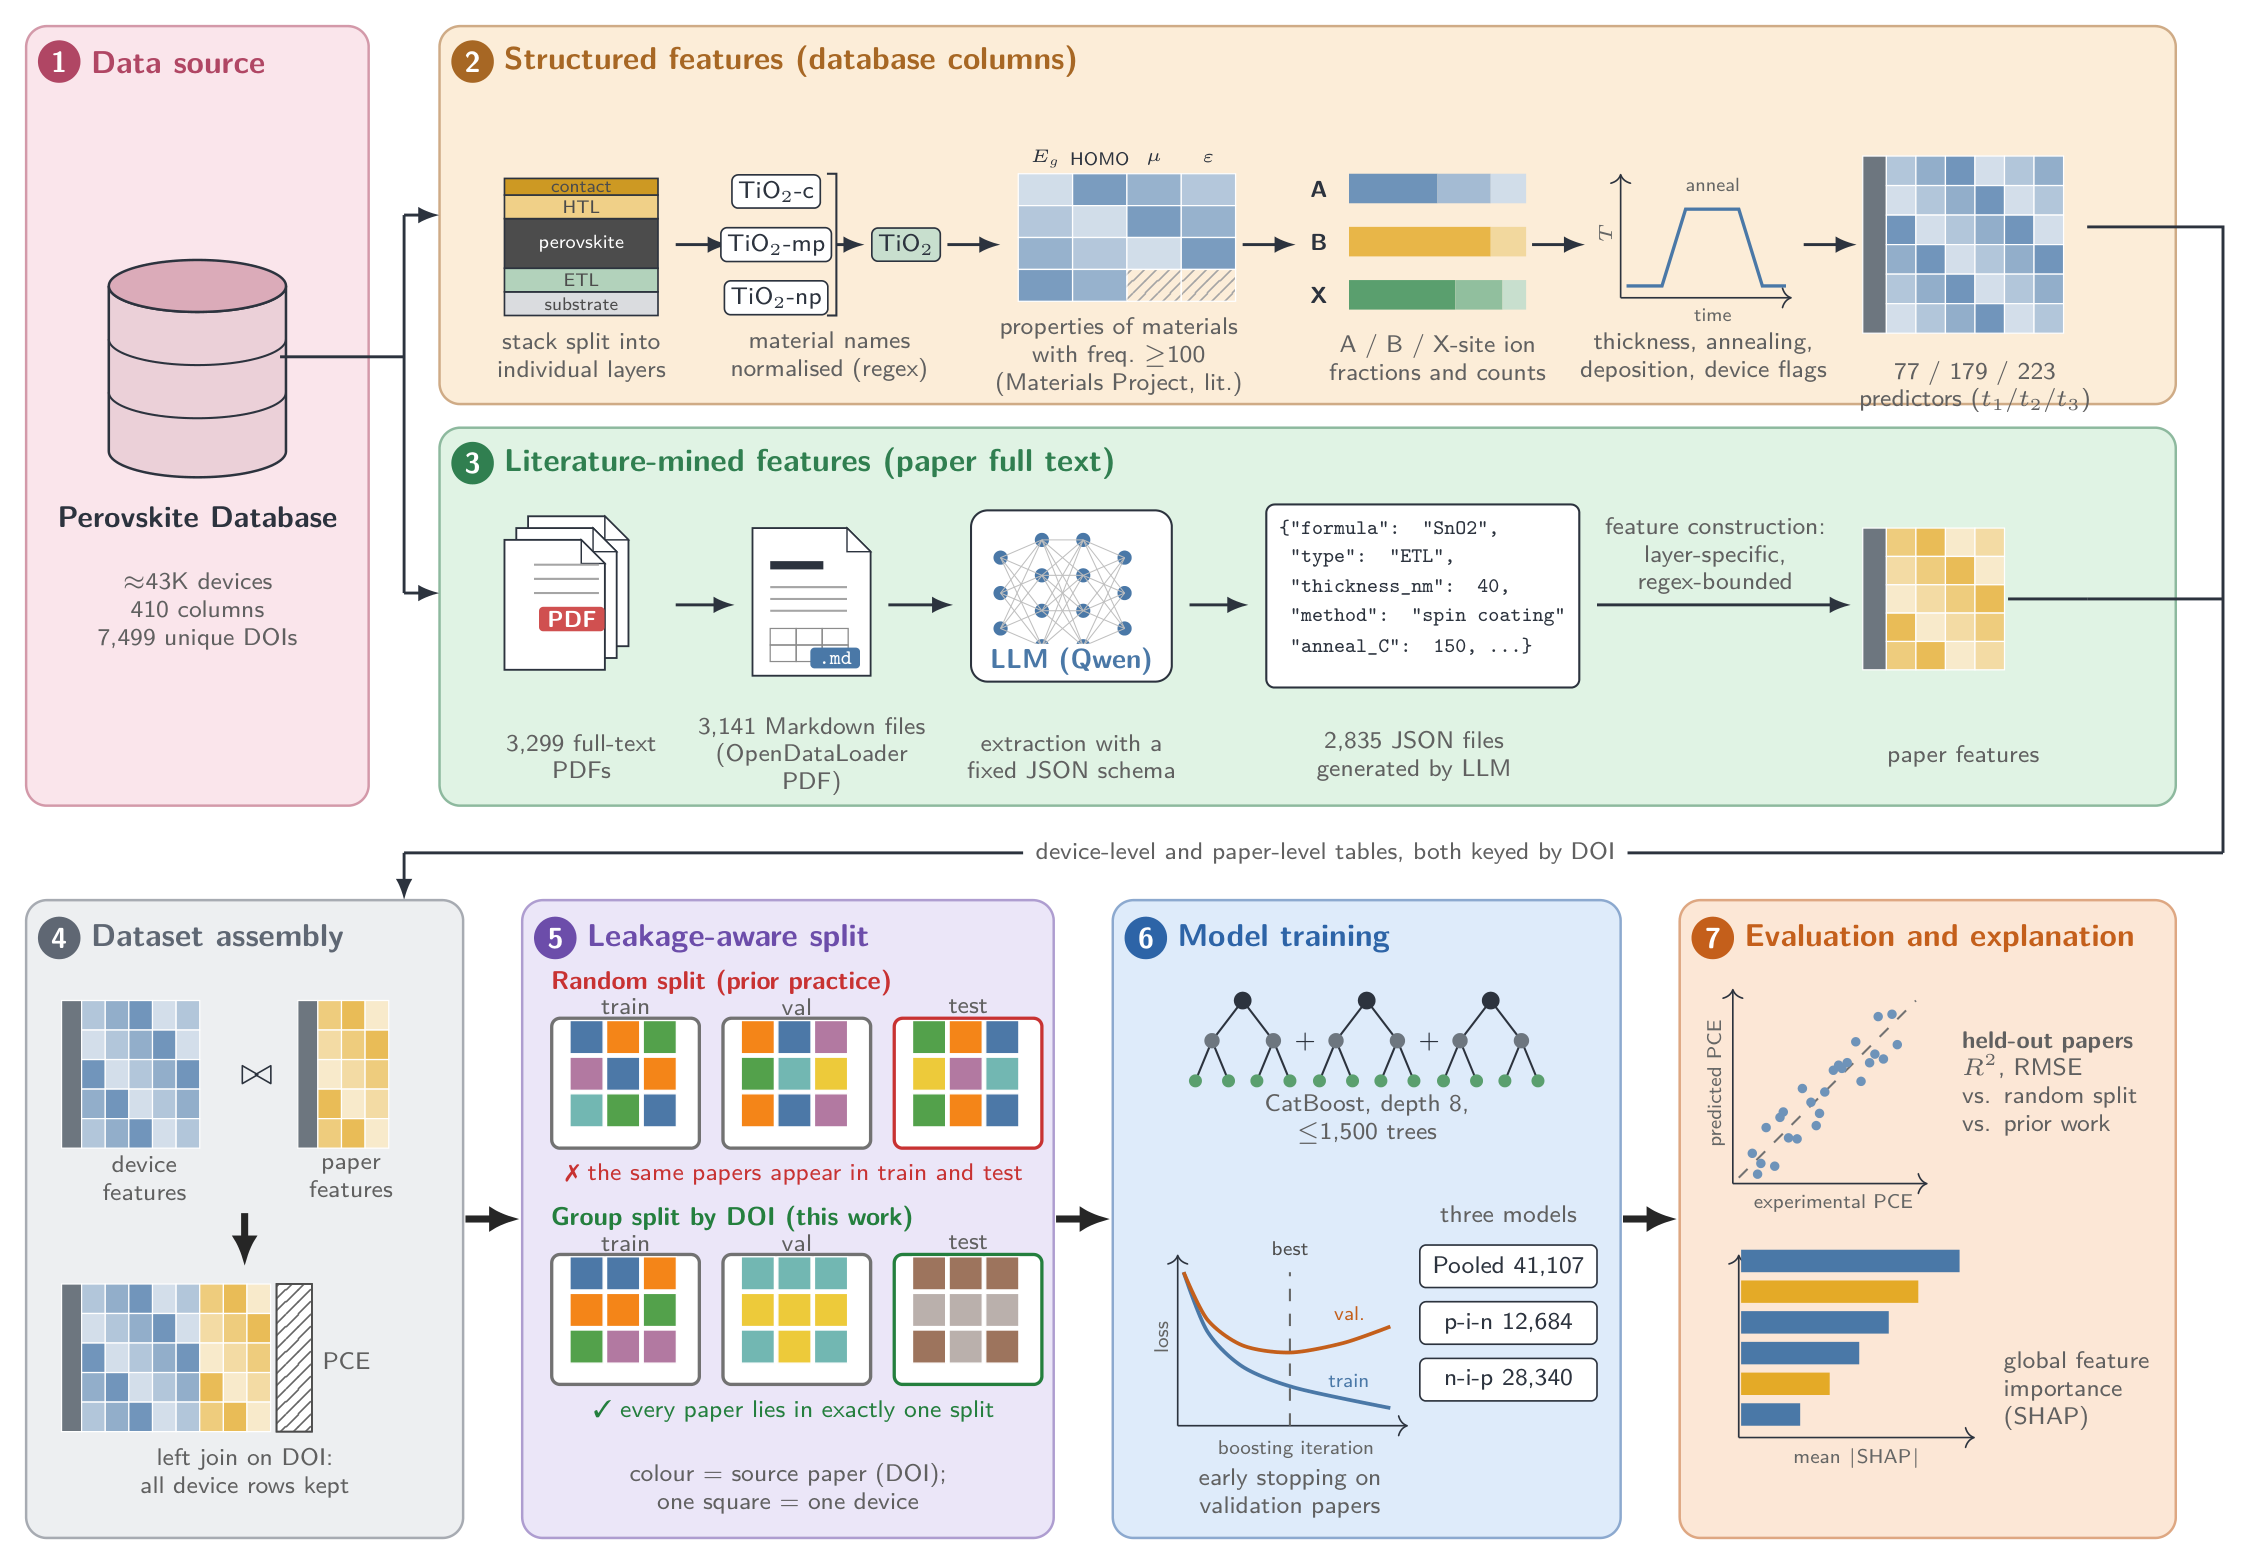
\includegraphics[width=\textwidth]{figures/ml_pipeline.png}
    \caption{Overview of the machine-learning workflow for perovskite solar-cell power conversion efficiency (PCE) prediction. The Perovskite Database Project provided unique DOIs, from which full-text PDFs were retrieved, which were converted to Markdown. Subsequently structured JSON files were generated through large language model (LLM)-based extraction. The resulting literature-derived features were integrated with structured database descriptors at the DOI level, followed by publication-grouped model evaluation using CatBoost and model interpretation using SHAP.
    Panel 6 shows the matched CatBoost configuration and the subset sizes used.}
    \label{fig:ml_workflow}
\end{figure}

% ---------------- METHODOLOGY ----------------
\section{Methods}

\subsection{Data Preparation}

\subsubsection{Dataset Description}

The Perovskite Database Project (PDP) is an open-access repository of experimentally reported perovskite solar cell (PSC) data, encompassing material compositions, device architectures, fabrication procedures, and photovoltaic characteristics \cite{jacobsson2022open}. The database export used in this study contained 43,398 device records, associated with 7,499 unique DOIs, and 410 columns. These records comprise heterogeneous data types, including categorical descriptions of functional layers, perovskite compositions, numerical device parameters, and fabrication-related variables. Previous PDP-based studies have demonstrated that appropriate data selection, cleaning, and representation are important for developing predictive models from these heterogeneous records \cite{roberts2024machine,fukasawa2024effectiveness}.

Five fields were initially extracted to construct the layer-resolved material representation: \texttt{ETL\_stack\_sequence}, \texttt{HTL\_stack\_sequence}, \texttt{Perovskite\_composition\_short\_form}, \texttt{JV\_default\_PCE}, and \texttt{Cell\_architecture}. These fields describe the electron transport layer (ETL), hole transport layer (HTL), perovskite composition, experimentally reported power conversion efficiency (PCE), and device architecture, respectively. The PCE field was renamed \texttt{final\_pce} for consistency throughout the processing pipeline, while the architecture field was retained for pooled modelling and architecture-specific analysis. This five-column extract was an intermediate representation for material processing rather than the complete predictor matrix; additional device and fabrication variables were retained from the original database for subsequent feature construction. Publication metadata, including DOI identifiers and author information, were excluded from the predictive feature set, while DOI identifiers were retained separately for linking records to the literature corpus and defining publication-level data partitions.

\subsubsection{Layer-Stack Parsing and Material Catalogue}

The material-stack descriptions in the PDP are stored as strings containing multiple materials or sequential layers, with vertical bars (\texttt{|}) delimiting successive entries. These strings were parsed into position-indexed fields, such as \texttt{ETL\_1}, \texttt{HTL\_1}, and \texttt{Perovskite\_1}, making the constituent materials independently accessible. The resulting representation accommodated up to seven ETL entries, three HTL entries, and five perovskite-layer entries. Where an entry contained multiple semicolon-separated materials, the individual materials were expanded into separate fields while preserving the recorded stack order. Material identifiers were also normalized by consolidating selected naming variants into common identifiers, facilitating consistent matching across device records.

A catalogue of unique standardized material identifiers was subsequently constructed from the parsed ETL, HTL, and perovskite fields. The catalogue contained 2,817 unique material identifiers, and the occurrence frequency of each identifier was calculated by counting its appearances across the parsed stack fields. This catalogue provided a common reference for material-level property retrieval and the construction of layer-specific descriptors (Section~\ref{sec:matprop}). The parsed identifiers were used for property lookup and were not themselves supplied to the models as categorical predictors.

\subsection{Literature Corpus Construction}

\subsubsection{DOI Identification and Full-Text Retrieval}

To enrich the structured device database with information from the original experimental literature, publication identifiers were extracted from the \texttt{Ref\_DOI\_number} field of the PDP. In total, 7,499 unique DOIs were identified across the 43,398 device records (7,326 publications plus 232 records without a DOI after the record filtering described in Section~\ref{sec:integration}). These identifiers were used to drive an automated full-text retrieval workflow, with retrieved documents associated with their corresponding DOIs to maintain traceability throughout subsequent processing. The retrieval workflow released with this work requests full texts only through legal routes, in order: open-access PDF locations listed by Unpaywall and OpenAlex, openly accessible publisher full-text links deposited with Crossref, and finally manual download through institutional access; each retrieval is logged with its route (\texttt{scripts/retrieve\_fulltext.py}). Retrieved PDFs, their Markdown conversions and the raw LLM outputs are not redistributed. The retrieval stage yielded 3,299 PDF documents. As full-text availability and successful retrieval varied across publications, the resulting corpus represented the subset of identified publications for which PDF documents were obtained.

\subsubsection{PDF Conversion and LLM-Based Information Extraction}
\label{sec:extraction}

The retrieved PDF documents were converted individually into Markdown using OpenDataLoader PDF, an open-source PDF parsing tool designed to produce machine-readable representations of document content and structure \cite{opendataloaderpdf}. This conversion yielded 3,141 Markdown documents from the 3,299 retrieved PDFs. The resulting files provided a text-based representation of each publication for subsequent processing by a large language model (LLM).

Each Markdown document was supplied individually to a locally served Qwen3.5-9B model (OpenAI-compatible vLLM endpoint, model alias \texttt{qwen35}, temperature 0.1, at most 16,384 output tokens; the exact checkpoint and quantisation are not recorded in the project files) using a predefined system prompt (reproduced in the Supplementary Information) and a structured JSON schema to guide consistent information extraction. The recovered extraction script is zero-shot; whether additional examples were used for the 2,835 outputs cannot be verified, so no few-shot claim is made. The extraction procedure was designed to identify reported materials and their functional classifications, together with available material properties, units, uncertainties, and measurement methods. Fabrication-related information, including deposition techniques, spin-coating parameters, annealing conditions, and processing environments, was also extracted where reported. Photovoltaic performance information was collected separately, with champion and average performance values distinguished where possible. The resulting structured outputs retained their association with the source DOI for subsequent paper-level feature construction.

The individual extraction outputs were consolidated into a combined JSON representation and subsequently organized into DOI-indexed JSON files. This process yielded 2,835 structured paper records. These records served as the intermediate representation for downstream feature construction, in which the extracted information was normalized and converted into a consistent set of publication-level descriptors for integration with the device-level database.

No hand-annotated reference set was available, so a true extraction precision/recall and hallucination rate were \emph{not} measured. As a proxy we compared the extracted features with the independently curated PDP entries for the same publications (\texttt{results/extraction\_validation.json}). For the numerical parameters, the paper-level value agreed with the median PDP device value within 10\% for 59--85\% of publications that have both (Spearman 0.44--0.90; perovskite thickness 0.79, $n=507$; annealing temperature 0.71, $n=455$), and for the material flags the DOI-level precision/recall against the PDP stack strings were 0.94/0.82 (TiO$_2$), 0.95/0.80 (Spiro-OMeTAD), 0.82/0.87 (PEDOT), 0.85/0.83 (NiO$_x$), 0.83/0.83 (PTAA) and 0.54/0.82 (SnO$_2$), with lower precision where the PDP records only a subset of the materials a paper describes (the BCP and LiF flags cannot be assessed because the PDP stack strings rarely contain those layers). This is agreement with a second human-curated source, not accuracy against ground truth. Importantly, the extracted numerical values equal the PDP value exactly in 59--82\% of records where both exist, and they supply a value where the PDP column is empty for only 0.8--5.3\% of records, so they are largely redundant with columns already present in $t_1$. The corpus shrank from 3,299 retrieved PDFs to 3,141 Markdown documents and 2,835 structured paper records; these matched 2,726 distinct DOI strings of the filtered dataset (2,699 publications after DOI normalisation), covering 14,896 of 41,107 records (36.2\%). Within the table, the literature features are non-missing exactly for publications with an extraction record (individual sparsely reported process parameters have lower coverage, 3.7--36.2\%) and, where present, are constant within a publication (\texttt{results/feature\_audit.json}, Supplementary Table~S4).

\subsubsection{DOI-Level Feature Construction}

The structured JSON records were parsed to construct a tabular dataset of publication-level features for integration with the device database. An initial, broader feature representation was developed and subsequently refined to retain information relevant to PSC materials and fabrication. The feature-construction procedure used recursive traversal of nested JSON objects to retrieve property values and associated units, together with normalization of synonymous field names and material-type labels. This harmonization enabled information expressed using different terminology across publications to be mapped to consistent feature definitions.

The resulting features represented material properties and fabrication conditions reported in the source literature, including layer-specific properties, deposition parameters, annealing conditions, and available processing-environment information. Material and layer assignments were resolved using standardized material classifications and bounded pattern matching to reduce false matches between similar material names. Layer-specific descriptors were retained separately rather than averaging properties across different functional layers. In addition to these material and processing descriptors, the table includes extraction-level descriptors, such as the number of numerical values recovered from a paper, which summarize how completely a publication reports its experimental details. Bibliographic metadata, including author names, journal names, and publication year, were excluded.

The final DOI-level feature table contained one row per successfully processed publication. These features represented information extracted from the associated research paper and were therefore defined at the publication level, rather than as independent measurements for every device reported in that paper. The table was subsequently linked to the device-level dataset by DOI.


\subsection{Feature Engineering}

\subsubsection{Composition-Derived Descriptors}

Composition-derived descriptors were constructed to represent the elemental and ionic composition of the perovskite absorber numerically. These features included the fractions of constituent ions at the A, B, and X sites and corresponding ion counts.

In addition to the site-specific composition descriptors, the feature set included composition-derived descriptors representing the average atomic mass and ionic radius of the perovskite absorber. The feature \texttt{Perovskite\_avg\_atomic\_mass} was calculated as a stoichiometric average of the atomic masses of the constituent elements. For a composition containing \(k\) constituent elements, this descriptor is defined as

\[
\overline{M}=\frac{\sum_{i=1}^{k} n_i M_i}{\sum_{i=1}^{k} n_i},
\]

where \(n_i\) is the stoichiometric coefficient of element \(i\) in the composition and \(M_i\) is its atomic mass. Consequently, the descriptor represents the average atomic mass weighted by the elemental stoichiometry rather than an unweighted average of the constituent atomic masses. It provides a compact numerical representation of compositional differences that can be used alongside the individual site-fraction and ion-count descriptors.

The feature \texttt{Perovskite\_avg\_radius} represents an average ionic-radius descriptor for the perovskite composition. It summarizes the ionic sizes associated with the constituent species and complements the site-specific composition descriptors by providing a scalar representation of the composition's characteristic ionic size. The resulting values depend on the ionic-radius reference data and the weighting procedure used during feature construction.

The feature \texttt{perovskite\_octahedral\_factor} represents a geometric descriptor of the perovskite composition. For an idealized \(ABX_3\) composition, the octahedral factor is defined as

\[
\mu=\frac{r_B}{r_X},
\]

where \(r_B\) and \(r_X\) are the ionic radii of the B-site cation and X-site anion, respectively. This ratio characterizes the relative sizes of the ions forming the \(BX_6\) octahedral framework. For mixed compositions, its calculation depends on how the effective B-site and X-site ionic radii are obtained from the constituent species. The octahedral factor was included as a composition-derived predictor; its inclusion does not, by itself, establish structural stability or a causal relationship with power conversion efficiency.

\subsubsection{Material-Property Augmentation}
\label{sec:matprop}

A separate material-property reference dataset was curated for standardized material identifiers with an occurrence frequency of at least 100 across the parsed ETL, HTL, and perovskite stacks. Available electronic and physicochemical properties were compiled from published literature and, where applicable, retrieved through the Materials Project database \cite{jain2013materialsproject}. These values represent general material-level reference properties rather than measurements reported for the specific PSC devices in which the materials appeared. Property availability was heterogeneous, and not every material had a complete set of descriptors.

The curated property catalogue included band gap, highest occupied molecular orbital (HOMO) energy, lowest unoccupied molecular orbital (LUMO) energy, electron mobility, hole mobility, dielectric constant, and material classification, together with the material identifier and occurrence frequency. Source references were associated with the curated values to support traceability.

For each device, property lookup was performed separately for the ETL, HTL, and perovskite layers. Within each layer family, the recorded material entries were traversed in their original order, and the first available non-missing value was assigned for each property. This procedure produced descriptors such as \texttt{ETL\_band\_gap}, \texttt{HTL\_HOMO}, and \texttt{Perovskite\_dielectric\_constant}. Because the lookup was performed independently for each property, the material supplying one descriptor was not necessarily the same material supplying another descriptor for a given layer family. Missing property values were retained during this stage and handled during model feature preparation.

\subsubsection{PDP-Derived Process and Device Features}

The composition descriptors were combined with relevant device and fabrication variables retained from the original PDP export. These variables included available layer-thickness information, deposition methods and solvents, annealing conditions, and device-related flags. Because the parsed material identifiers were not used as predictors, this database-level representation ($t_1$, Section~\ref{sec:tiers}) contains no explicit information on which transport-layer materials were used; that information enters the model only through the material-property descriptors of $t_2$.

\subsubsection{LLM-Derived Literature Features}

The DOI-level feature table was used to augment the device-level representation with information extracted from the associated research papers. Paper-level features were not treated as device-specific experimental measurements; instead, they provided publication-level context derived from the reported literature. The feature-construction process normalized aliases and functional classifications before producing the final DOI-level table, allowing the same feature definitions to be applied consistently across publications. Photovoltaic outcome fields extracted during literature processing were not used as model predictors. The 32 literature-derived base columns (44 predictors once their missingness indicators are included) are listed in Table~S1 of the Supplementary Information. Because several of them describe how completely a paper reports its methods (e.g.\ \texttt{json\_numeric\_values\_found}, \texttt{has\_stability\_measurement}), they can act as proxies for the publication itself; Section~\ref{sec:features} tests their contribution with controls.

\subsubsection{Recipe-flag block (final LLM-derived representation).}
\label{sec:recipe}
The final LLM-derived representation, denoted $t_3$, was built from the same stored extraction JSON (no new LLM calls and no further full-text retrieval) by deterministic matching of canonicalised material names and process fields. It consists of 36 binary paper-level recipe flags (\texttt{rc\_*}): additive and precursor identities (for example chloride and thiocyanate sources, acetate, SnF$_2$, 5-AVA, hydrohalic acids, alkali and Cs additives, PEA-family spacers, Lewis bases, polymer, water and DIO additives, carbon-based contacts), electron- and hole-transport-layer dopants and treatments (TBP, LiTFSI, FK-type dopants, F4-TCNQ, Cu salts, borates, TiCl$_4$, undoped layers, interface passivation), process route (antisolvent, vacuum, two-step, hot casting, solvent annealing, nitrogen box versus ambient) and device context (flexible, tandem, lead-free, inorganic, mesoscopic). $t_3$ is $t_2$ plus these flags. The flags are missing for publications without an extraction record, which covers 15,027 of 41,107 records (36.6\%; 2,731 publications), and a CatBoost first-feature-use penalty of 0.5 is applied to these columns. Photovoltaic outcome fields were not used. The flags are paper-level outputs of pattern matching over LLM-extracted JSON, so they are noisy and cannot distinguish devices within a publication. The original 44-predictor block described above, denoted simply $t_3^{\mathrm{orig}}$ in the controlled ablation (Tables~\ref{tab:tiers}--\ref{tab:groups} and Figs.~\ref{fig:tiers}--\ref{fig:groups}), is a different representation and is not a subset of $t_3$.

\subsection{Data Integration, Filtering and Feature Tiers}
\label{sec:integration}

The structured device-level feature table and the DOI-level literature feature table were integrated using the publication DOI as the join key. DOI strings were normalised before matching and before grouping by removing byte-order marks and whitespace, lower-casing, and stripping \texttt{doi.org} and \texttt{doi:} prefixes; this merges 45 case/prefix variants, so the 7,371 raw DOI strings of the filtered data correspond to 7,326 publications. A left join was performed from the device-level table to the DOI-level feature table, retaining the device records even when a corresponding literature-feature record was unavailable. Missing paper-level features arising from unsuccessful retrieval, incomplete extraction, or unmatched DOI identifiers were preserved as missing values for subsequent model preparation.

The initial PDP export contained 43,398 records associated with 7,499 unique raw DOI strings. We excluded 1,002 records with missing target values and a further 1,289 records with reported PCE below 1.0\%, giving 41,107 records from 7,326 publications plus 232 records without a DOI (Table~\ref{tab:dataset}). Of these, 28,340 records were n-i-p and 12,684 were p-i-n devices; the remaining 83 records have other or unspecified architectures and were used only in the pooled model. The filtered set contains 17 records (six publications) with PCE above 27\%, i.e.\ above the certified single-junction record; the enriched table carries no illumination or tandem field with which to remove them on physical grounds, so they were retained under the pre-declared filter. Excluding them from the test sets changes the pooled $t_3^{\mathrm{orig}}$ $R^2$ by $+0.002$ (0.407 to 0.409), so they do not drive any conclusion. The DOI was used exclusively as a record-linkage and grouping variable and was never a predictor. The 232 records without a DOI were treated as one explicit group that is never divided between partitions; this is conservative, because their true publications are unknown. Free-text columns were removed. All data-dependent preprocessing was fitted on the training partition of each split only: columns with more than 80\% missing values were dropped, numerical features with missing entries were median-imputed and accompanied by a binary missingness indicator (suffix \texttt{\_na}), and missing categorical features were assigned the label ``unknown''. The predictor columns of each tier are listed in the Supplementary Information (Table~S1).

\begin{table}[t]
    \centering\small
    \caption{Summary of the dataset used for modelling.}
    \label{tab:dataset}
    \begin{tabular}{lr}
        \toprule
        Quantity & Value \\
        \midrule
        Records in PDP export (raw DOI strings) & 43,398 (7,499) \\
        Removed: missing PCE & 1,002 \\
        Removed: PCE $<$ 1.0\% & 1,289 \\
        Records after filtering (publications) & 41,107 (7,326) \\
        \quad n-i-p / p-i-n / other architecture & 28,340 / 12,684 / 83 \\
        \quad Records without DOI & 232 \\
        Records with LLM-derived literature features (publications) & 14,896 (2,699) \\
        PCE after filtering: mean, median, range (\%) & 12.4, 13.0, 1.0--36.2 \\
        Records per publication: median, maximum & 4, 127 \\
        Target variance between publications (ICC) & 0.69 \\
        \bottomrule
    \end{tabular}
\end{table}

\subsection{Machine Learning Models and Evaluation}

\subsubsection{Prediction task and feature tiers.}
\label{sec:tiers}
We formulated PCE prediction as a supervised regression task, with experimentally reported PCE as the target. Three nested feature tiers were defined (Table~\ref{tab:tiertable}): the PDP database representation ($t_1$), comprising device architecture, layer deposition and fabrication variables and composition-derived descriptors; $t_1$ augmented with material-property descriptors ($t_2$); and $t_2$ further augmented with the original block of LLM-derived literature features ($t_3^{\mathrm{orig}}$). Nesting is enforced in code and asserted in the test suite. Each tier was evaluated on the pooled dataset and separately on the p-i-n and n-i-p subsets, which were modelled independently. Three additional control tiers were used only to probe the literature features: $t_1$ plus the literature block without material properties; $t_3^{\mathrm{orig}}$ without the two reporting-completeness flags (\texttt{json\_numeric\_values\_found}, \texttt{has\_stability\_measurement}); and $t_2$ plus 32 columns of N(0,1) noise (a negative control). The final recipe-flag representation ($t_3$, Section~\ref{sec:recipe}) is not part of this ablation; it is evaluated separately on reserved publications (Section~\ref{sec:recipe_results}).

\begin{table*}[t]
    \centering\small
    \caption{Feature tiers. Counts are for the pooled model and include missingness indicators. Because the indicator set is derived from each training partition, the n-i-p and p-i-n models contain on average 76/178/222 and 77/179/224 features for $t_1$/$t_2$/$t_3^{\mathrm{orig}}$. Exact lists: Supplementary Table~S1.}
    \label{tab:tiertable}
    \begin{tabular}{llrp{8cm}}
        \toprule
        Feature group & Tier & No. of features & Content \\
        \midrule
        Process & $t_1$ & 21 & Deposition methods, annealing, layer thickness \\
        Device & $t_1$ & 9 & Architecture and device flags \\
        Composition & $t_1$ & 47 & A-, B- and X-site ion fractions and counts \\
        Material properties & $t_2$ & 102 & Band gap, HOMO/LUMO, mobility, etc.\ (49 base columns plus 2 band-alignment differences and indicators) \\
        Literature (LLM) & $t_3^{\mathrm{orig}}$ & 44 & 32 paper-level base columns plus indicators \\
        \midrule
        Total & $t_1$ / $t_2$ / $t_3^{\mathrm{orig}}$ & 77 / 179 / 223 & \\
        \bottomrule
    \end{tabular}
\end{table*}

\subsubsection{Model training.}
\label{sec:models}
Models were trained with CatBoost \cite{prokhorenkova2018catboost}, using its native handling of the categorical variables (architecture and the deposition methods). To ensure a controlled comparison across feature tiers, all three tiers used a single CatBoost regressor with the same fixed hyperparameters (Table~\ref{tab:config}). These values were fixed a priori and inherited from an earlier configuration of this project that was not tuned in the present study; the number of trees was chosen by early stopping on a DOI-disjoint validation set and no tier was tuned. The only difference between tiers is the predictor set, so the tier comparisons are feature ablations rather than comparisons between model architectures, hyperparameters or ensembling. Reference models were trained on the same splits and features: a training-mean predictor; ridge regression (one-hot categorical encoding, standardised and winsorised numerical features, penalty chosen on the validation set); XGBoost with library defaults (the setting of Roberts-style pipelines); a random forest (300 trees); a multilayer perceptron (two hidden layers, early stopping on the validation set); and an exact Gaussian process on a fixed random subsample of 3,000 training records (exact GPR scales cubically with the number of records). A separate model-development experiment on the original-block tiers, \emph{not} used for the tier comparison, selected CatBoost depth and L2 regularisation from a six-point grid by validation RMSE (identical grid for every tier), then averaged three seeds, and combined this bag with an early-stopped XGBoost model.

\begin{table*}[t]
    \centering\small
    \caption{Matched CatBoost configuration used for all tiers, splits and protocols.}
    \label{tab:config}
    \begin{tabular}{p{7.4cm}p{7.4cm}}
        \toprule
        Setting & Value \\
        \midrule
        Loss, learning rate, depth & RMSE, 0.05, 8 \\
        Maximum iterations, early stopping & 1,500 (6,000 for the record-level arm, see text), 100 rounds on the validation set \\
        L2 regularisation, row subsample, feature subsample per level & 3.0, 0.8, 0.7 \\
        Minimum data in leaf, seed & 5, 42 \\
        \bottomrule
    \end{tabular}
\end{table*}

\subsubsection{Evaluation protocol with a DOI-disjoint validation set.}
To evaluate generalization to previously unseen publications, we used five repeated DOI-grouped holdout splits generated with \texttt{GroupShuffleSplit} (test fraction 0.2 of publications, seed 42), so that records sharing a normalised DOI were always assigned to the same partition (Table~\ref{tab:protocol}). Within each training partition, a further DOI-disjoint validation set (15\% of the training publications) was used for early stopping and, where applicable, model selection; the test partition was used only for the final evaluation, and the model was not refitted on the validation records. No DOI occurs in more than one of the training, validation and test partitions in any split; this is recorded in every run record and checked by automated tests. Because repeated group-shuffle splits may have overlapping test sets, the evaluation is a repeated DOI-grouped holdout evaluation rather than mutually exclusive five-fold cross-validation, and the standard deviations reported across splits describe split-to-split variability rather than confidence intervals. The record-level comparison protocol used \texttt{ShuffleSplit} with the same fractions, seed scheme, tiers, preprocessing and models; its validation set is a random subset of the training records. Record-level fits keep improving on a random validation set for much longer than DOI-grouped fits (a first run with the 1,500-iteration cap truncated 31 of 45 record-level CatBoost fits). The record-level arm was therefore rerun with a cap of 6,000 iterations for all subsets, and for the pooled data again with a cap of 20,000 iterations, where all 15 fits stopped on their own (best iteration 7,207--11,702); the pooled record-level numbers reported here are the converged ones. DOI-grouped fits stop before 500 iterations and are unaffected by the cap. Two stricter protocols were run for the pooled and architecture-specific models with the same tiers, preprocessing, models and validation scheme. \emph{Lead-author grouping} assigns each publication the modal PDP lead-author surname (a proxy for laboratory; common surnames such as Wang, Zhang and Li make some groups large and heterogeneous, so this over-groups) and splits by that key with the same \texttt{GroupShuffleSplit} settings; records without DOI remain one block. \emph{Forward-in-time splitting} dates each publication by its earliest PDP record and, for three non-overlapping test windows covering publication-date quantiles (0.55, 0.70], (0.70, 0.85] and (0.85, 1.00] (test dates 2018-05 to 2024-08), trains on strictly earlier publications, with the most recent 15\% of those as validation set; all partitions are DOI-disjoint by construction. Paired differences between tiers were assessed within each split by a cluster bootstrap that resamples test publications with replacement (1,000 resamples) and reports the per-split 95\% percentile interval; because the test sets of different repeats overlap, no pooled significance test is reported.

\begin{table*}[t]
    \centering\small
    \caption{Data-splitting protocol (pooled dataset; means over five splits).}
    \label{tab:protocol}
    \begin{tabular}{p{5.6cm}p{9.4cm}}
        \toprule
        Item & Setting \\
        \midrule
        Grouping variable & Normalised publication DOI; records without DOI form one block \\
        Splitter & \texttt{GroupShuffleSplit}, 5 repeats, seed 42 (inner split seed 42$+k$) \\
        Training set & about 27,700 records, 4,981 publications \\
        Validation set (15\% of training publications) & about 5,000 records, 880 publications; early stopping/model selection only \\
        Test set (20\% of publications) & about 8,430 records, 1,466 publications \\
        DOI overlap, train/validation/test & Zero in every split and partition pair \\
        Comparison protocol & Record-wise \texttt{ShuffleSplit}, same fractions and seeds \\
        Reported statistics & Mean $\pm$ s.d. over the five splits \\
        \bottomrule
    \end{tabular}
\end{table*}

\subsubsection{Evaluation of the recipe-flag block.}
\label{sec:v4protocol}
The recipe-flag block was evaluated under a separate protocol fixed after the controlled ablation. Publications were assigned by a salted DOI hash to a development partition (65\%; 26,982 records, 4,708 publications) used for all design, tuning and ablation work, and a reserved partition (35\%; 14,125 records, 2,619 publications, of which 5,460 records from 1,005 publications have extraction data) scored once. The reserved publications had appeared in earlier experiments with other feature representations, so they are new for this representation but not untouched data, and the flag block was selected after comparisons on development publications. For $t_2$ and $t_3$ separately, an equal-budget random search of 24 CatBoost configurations (the matched default included) was scored by DOI-grouped five-fold mean squared error on development publications. For the final scoring, models were trained on all development records (DOI-disjoint 15\% validation set for early stopping), five seed models were averaged, and paired differences on the reserved publications were assessed by a publication-cluster bootstrap of the squared error (2,000 resamples). Two comparisons isolate different questions: \emph{same settings} gives both tiers the matched default configuration (or both the same tuned configuration), so that only the added features differ; \emph{each tuned} gives each tier its own selected configuration. Negative controls replaced the flag block by five DOI-permuted copies or by a coverage indicator alone. Scores are reported for the covered subset (reserved records from publications with extraction data) and for all reserved records. Because this partition and protocol differ from the five repeated holdouts above, absolute $R^2$ values from the two protocols are not comparable.

\subsubsection{Performance metrics.}
Predictive performance was assessed using the coefficient of determination ($R^2$), mean absolute error (MAE), and root mean squared error (RMSE), calculated by comparing experimentally reported PCE values, $y_i$, with predictions, $\hat{y}_i$, for the $N$ records in each held-out test partition:
\begin{equation}
    R^2 =
    1-\frac{\sum_{i=1}^{N}(y_i-\hat{y}_i)^2}
    {\sum_{i=1}^{N}(y_i-\bar{y})^2},
\end{equation}
\begin{equation}
    \mathrm{MAE} =
    \frac{1}{N}\sum_{i=1}^{N}|y_i-\hat{y}_i|,
\end{equation}
\begin{equation}
    \mathrm{RMSE} =
    \sqrt{\frac{1}{N}\sum_{i=1}^{N}(y_i-\hat{y}_i)^2},
\end{equation}
where $\bar{y}$ is the mean experimentally reported PCE in the corresponding test partition. MAE and RMSE are expressed in PCE percentage points. The coefficient of determination measures performance relative to a constant-mean reference, whereas MAE and RMSE quantify absolute prediction errors, with RMSE assigning greater weight to large deviations.

\subsection{Feature Importance and Model Interpretation}

SHAP (Shapley additive explanations) was used to interpret the fitted CatBoost models and quantify the contributions of individual predictors to PCE predictions \cite{shappaper}. SHAP values were computed for the original-block ($t_3^{\mathrm{orig}}$) models, not for the recipe-flag models, with \texttt{TreeExplainer} for a random sample of 1,500 held-out records from the first DOI-grouped split, using the matched CatBoost model trained for $t_3^{\mathrm{orig}}$ with validation-based early stopping. Global feature importance was assessed using mean absolute SHAP values. The analysis was conducted for the pooled dataset and the separate p-i-n and n-i-p models, and features were aggregated into the groups of Table~\ref{tab:tiertable} to compare group-level contributions. Because the p-i-n and n-i-p models were trained on different records, differences between their rankings describe what each model learned rather than different physical effects in the two architectures.

% ---------------- RESULTS AND DISCUSSION ----------------
\section{Results and Discussion}

\subsection{Generalization to unseen publications}
\label{sec:generalization}

With the matched CatBoost configuration and all features ($t_3^{\mathrm{orig}}$), the pooled model reached $R^2 = 0.407 \pm 0.031$, MAE $= 2.96 \pm 0.08$ and RMSE $= 3.79 \pm 0.08$ percentage points on publications it had not seen (Table~\ref{tab:tiers}, Fig.~\ref{fig:tiers}; mean $\pm$ s.d. over five repeated DOI-grouped holdouts, each with a DOI-disjoint validation set for early stopping). The training-mean predictor has $R^2 \approx 0$ and MAE $4.08$, so the model removes about 28\% of the mean absolute error. Performance differed by architecture: $R^2$ was $0.405 \pm 0.010$ for n-i-p and $0.294 \pm 0.074$ for p-i-n devices, whereas MAE (2.96 and 3.05) and RMSE (3.82 and 3.95) were similar. The p-i-n result is also the less certain one, because the subset is smaller (about 2,600 test records and 451 test publications per split). Relative to the training-mean predictor, the p-i-n model reduces MAE by 21\% (3.84 to 3.05) and the n-i-p model by 28\% (4.11 to 2.96), so on this data p-i-n devices are somewhat harder to predict, in addition to $R^2$ depending on the PCE variance within each subset.

\begin{table}[t]
    \centering\small
    \caption{Performance across nested feature tiers with the same CatBoost configuration (Table~\ref{tab:config}) under repeated DOI-grouped holdout evaluation (mean $\pm$ s.d. over five splits; MAE and RMSE in PCE percentage points; $N$ is the mean number of test records per split; the number of features varies slightly between splits because the missingness indicators are derived from each training partition).}
    \label{tab:tiers}
    \begin{tabular}{llrrccc}
        \toprule
        Subset & Feature tier & $N$ & Feat. & $R^2$ & MAE & RMSE \\
        \midrule
        Pooled & Database only ($t_1$) & 8,428 & 77 & $0.368 \pm 0.024$ & $3.081 \pm 0.040$ & $3.908 \pm 0.046$ \\
        Pooled & + material ($t_2$) & 8,428 & 179 & $0.408 \pm 0.032$ & $2.950 \pm 0.080$ & $3.783 \pm 0.085$ \\
        Pooled & + material + orig.\ lit.\ ($t_3^{\mathrm{orig}}$) & 8,428 & 223 & $0.407 \pm 0.031$ & $2.958 \pm 0.080$ & $3.787 \pm 0.083$ \\
        \midrule
        p-i-n & Database only ($t_1$) & 2,598 & 77 & $0.244 \pm 0.058$ & $3.168 \pm 0.049$ & $4.085 \pm 0.114$ \\
        p-i-n & + material ($t_2$) & 2,598 & 179 & $0.291 \pm 0.065$ & $3.047 \pm 0.045$ & $3.955 \pm 0.131$ \\
        p-i-n & + material + orig.\ lit.\ ($t_3^{\mathrm{orig}}$) & 2,598 & 224 & $0.294 \pm 0.074$ & $3.051 \pm 0.067$ & $3.947 \pm 0.142$ \\
        \midrule
        n-i-p & Database only ($t_1$) & 5,612 & 76 & $0.374 \pm 0.016$ & $3.062 \pm 0.047$ & $3.918 \pm 0.061$ \\
        n-i-p & + material ($t_2$) & 5,612 & 178 & $0.404 \pm 0.013$ & $2.966 \pm 0.036$ & $3.825 \pm 0.060$ \\
        n-i-p & + material + orig.\ lit.\ ($t_3^{\mathrm{orig}}$) & 5,612 & 222 & $0.405 \pm 0.010$ & $2.964 \pm 0.017$ & $3.821 \pm 0.045$ \\
        \bottomrule
    \end{tabular}
\end{table}

\begin{figure}[t]
    \centering
    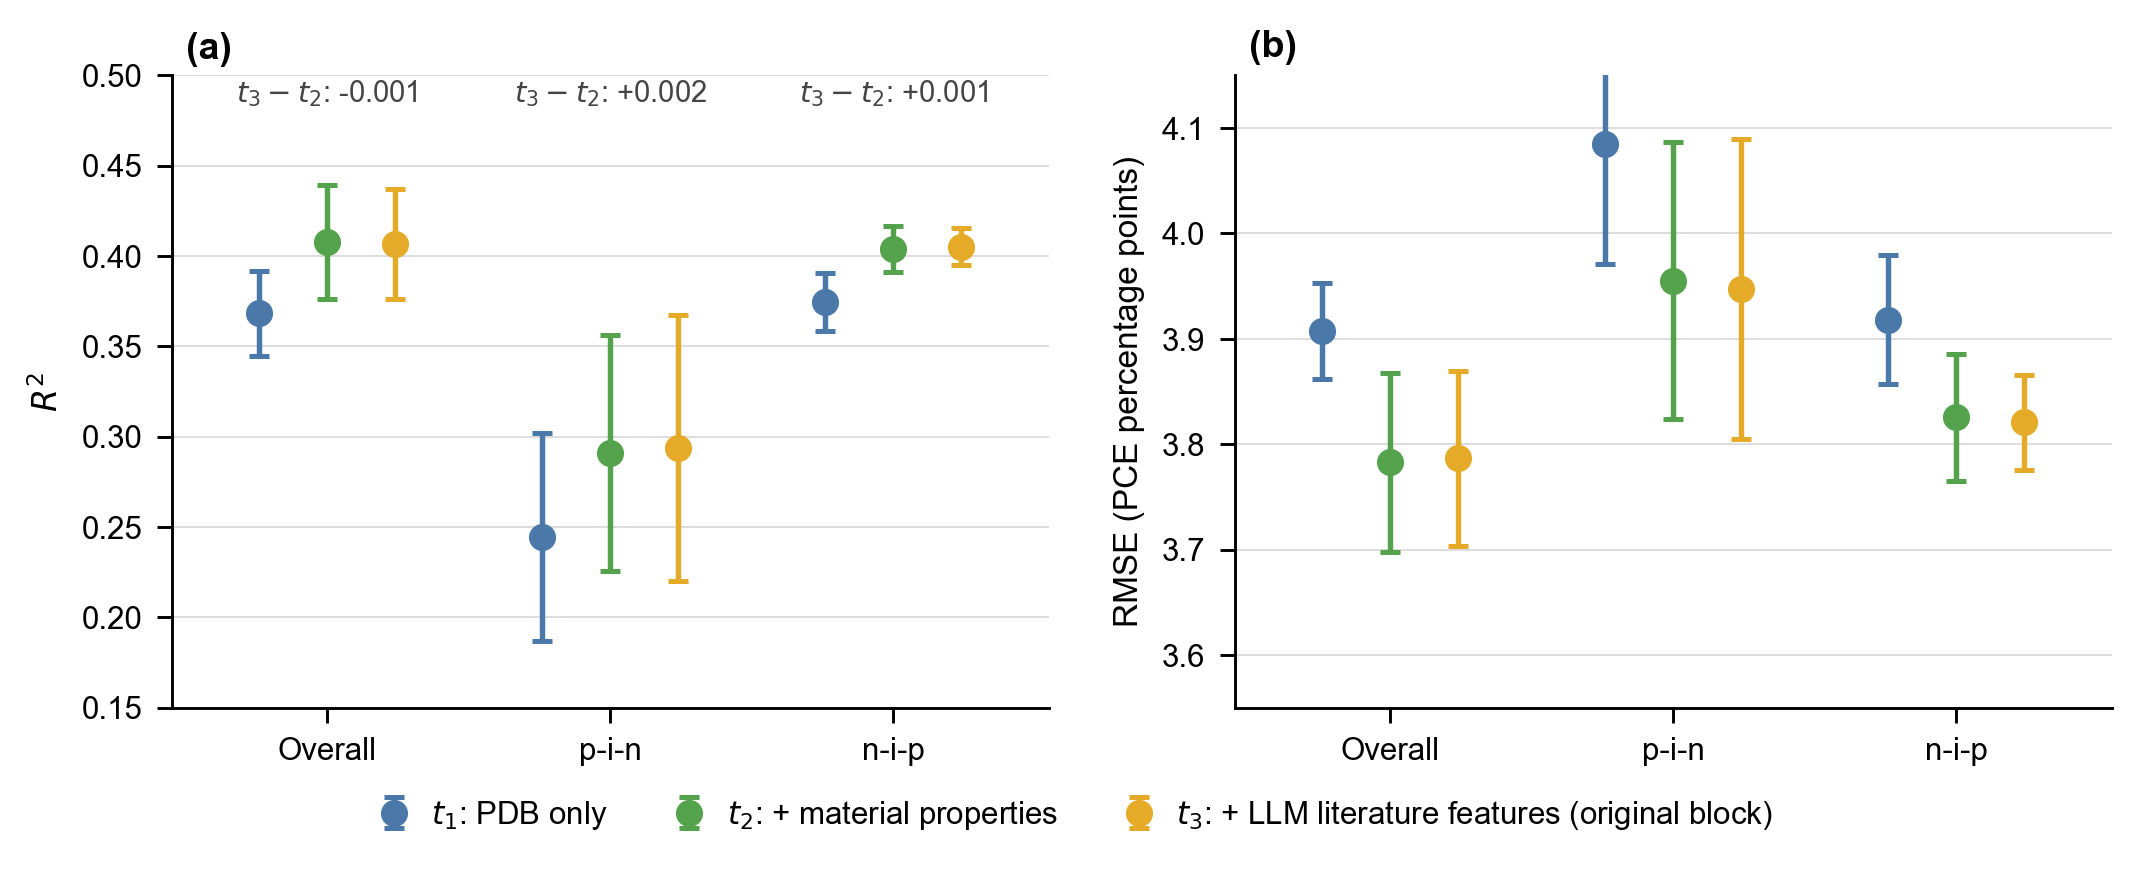
\includegraphics[width=\textwidth]{figures/fig_feature_tiers.png}
    \caption{Effect of feature tier on prediction of unseen publications (matched CatBoost, DOI-grouped splits). (a) $R^2$ and (b) RMSE, mean $\pm$ s.d. over five holdout splits; the vertical axes are truncated to the plotted range. $t_3^{\mathrm{orig}}$ is the original literature block, and the recipe-flag block is evaluated separately in Fig.~\ref{fig:v4}. The $t_1\!\to\!t_2$ step is visible in all subsets; the $t_2\!\to\!t_3^{\mathrm{orig}}$ step (original literature block) is not distinguishable from zero.}
    \label{fig:tiers}
\end{figure}

The pooled results should be read against simple references (Table~\ref{tab:baselines}). Ridge regression on the same $t_3^{\mathrm{orig}}$ features reaches $R^2 = 0.350 \pm 0.033$, i.e.\ most of what CatBoost achieves, and XGBoost with library defaults, a random forest, a validation-early-stopped MLP and a subsample-trained Gaussian process lie between 0.35 and 0.38. Matched CatBoost is the best of these by 0.03 (XGBoost, MLP) to 0.06 (ridge, random forest, GPR) in $R^2$; the margin over XGBoost and the MLP is comparable to the split-to-split standard deviation (0.02--0.03), so we do not claim a ranking among the non-linear models. A properly trained MLP and a Gaussian process are thus competitive with the tree ensemble on this dataset. All reference models improve when the material and literature blocks are added ($t_1\!\to\!t_3^{\mathrm{orig}}$), consistent with the CatBoost ablation.

\begin{table}[t]
    \centering\small
    \caption{Reference models on the pooled dataset under the same five DOI-grouped splits (mean $\pm$ s.d.; MAE and RMSE in PCE percentage points). All models use validation data only for early stopping or penalty selection; XGBoost (defaults) and the random forest use no validation data. The Gaussian process is fitted to 3,000 randomly chosen training records.}
    \label{tab:baselines}
    \begin{tabular}{llccc}
        \toprule
        Model & Tier & $R^2$ & MAE & RMSE \\
        \midrule
        Training-mean predictor & $t_1$ & $-0.001 \pm 0.001$ & $4.079 \pm 0.036$ & $4.920 \pm 0.047$ \\
        Training-mean predictor & $t_3^{\mathrm{orig}}$ & $-0.001 \pm 0.001$ & $4.079 \pm 0.036$ & $4.920 \pm 0.047$ \\
        Ridge regression & $t_1$ & $0.307 \pm 0.030$ & $3.271 \pm 0.039$ & $4.093 \pm 0.064$ \\
        Ridge regression & $t_3^{\mathrm{orig}}$ & $0.350 \pm 0.033$ & $3.141 \pm 0.054$ & $3.963 \pm 0.078$ \\
        CatBoost (matched) & $t_1$ & $0.368 \pm 0.024$ & $3.081 \pm 0.040$ & $3.908 \pm 0.046$ \\
        CatBoost (matched) & $t_3^{\mathrm{orig}}$ & $0.407 \pm 0.031$ & $2.958 \pm 0.080$ & $3.787 \pm 0.083$ \\
        XGBoost (library defaults) & $t_1$ & $0.334 \pm 0.031$ & $3.148 \pm 0.052$ & $4.011 \pm 0.070$ \\
        XGBoost (library defaults) & $t_3^{\mathrm{orig}}$ & $0.377 \pm 0.025$ & $3.011 \pm 0.057$ & $3.880 \pm 0.056$ \\
        Random forest & $t_1$ & $0.295 \pm 0.018$ & $3.219 \pm 0.041$ & $4.128 \pm 0.058$ \\
        Random forest & $t_3^{\mathrm{orig}}$ & $0.352 \pm 0.021$ & $3.073 \pm 0.049$ & $3.958 \pm 0.070$ \\
        MLP (val. early stopping) & $t_1$ & $0.343 \pm 0.020$ & $3.144 \pm 0.029$ & $3.987 \pm 0.025$ \\
        MLP (val. early stopping) & $t_3^{\mathrm{orig}}$ & $0.376 \pm 0.023$ & $3.042 \pm 0.052$ & $3.883 \pm 0.056$ \\
        GPR (3,000-record subsample) & $t_1$ & $0.330 \pm 0.024$ & $3.197 \pm 0.039$ & $4.025 \pm 0.053$ \\
        GPR (3,000-record subsample) & $t_3^{\mathrm{orig}}$ & $0.352 \pm 0.029$ & $3.129 \pm 0.051$ & $3.957 \pm 0.065$ \\
        \bottomrule
    \end{tabular}
\end{table}

\subsubsection{Model development: strongest validated predictor.}
Separately from the controlled ablation, we asked how much a validation-tuned and ensembled model improves on the matched configuration (Table~\ref{tab:dev}). For each split and tier, CatBoost depth and L2 regularisation were selected from a six-point grid by validation RMSE (the same grid and budget for every tier), the selected configuration was averaged over three seeds, and the result was averaged with an early-stopped XGBoost model. The ensemble reached $R^2 = 0.418 \pm 0.026$, MAE $= 2.92$ and RMSE $= 3.75$ percentage points for the pooled $t_3^{\mathrm{orig}}$ data (p-i-n $0.300 \pm 0.074$, n-i-p $0.413 \pm 0.015$), 0.011 above the matched CatBoost. This gain comes from tuning, bagging and ensembling and not from any additional feature: the same pipeline gives 0.377, 0.416 and 0.418 for $t_1$, $t_2$ and $t_3^{\mathrm{orig}}$, so the $t_2\!\to\!t_3^{\mathrm{orig}}$ step remains negligible ($+0.002$) and the material-property step ($+0.039$) remains the only measurable feature effect. Because $t_2$ and $t_3^{\mathrm{orig}}$ are indistinguishable, the $t_2$ representation, which needs no full-text retrieval or LLM extraction, is the most economical predictor with this performance; we use $t_3^{\mathrm{orig}}$ numbers only where the full model is the object of study. The $t_3^{\mathrm{orig}}$ rows here and in the controlled ablation use the original literature block; the recipe-flag block was evaluated on a different partition with separately tuned CatBoost models (Table~\ref{tab:v4}), without bagging or ensembling, and those results neither replace nor can be merged into Table~\ref{tab:dev}. We regard $R^2 \approx 0.42$ and MAE $\approx 2.9$ percentage points as the performance on unseen publications supported by this evaluation, with the caveat that the split-to-split standard deviation is 0.03 and the validation-selected configuration changed between splits.

\begin{table}[t]
    \centering\small
    \caption{Model-development experiment (DOI-grouped splits; $R^2$, mean $\pm$ s.d. over five splits). Tuned: CatBoost with depth/L2 chosen on the validation set; Bag: three-seed average of the selected configuration; XGB: early-stopped XGBoost; Ens: mean of Bag and XGB. $t_3^{\mathrm{orig}}$ is the original literature block. This experiment differs from the matched ablation in estimator and budget, so it must not be used to attribute differences to features, and it is not the same experiment as the recipe-flag evaluation (Table~\ref{tab:v4}).}
    \label{tab:dev}
    \begin{tabular}{llcccc}
        \toprule
        Subset & Feature tier & Tuned & Bag & XGB & Ens \\
        \midrule
        Pooled & Database only ($t_1$) & $0.371 \pm 0.023$ & $0.372 \pm 0.023$ & $0.368 \pm 0.019$ & $0.377 \pm 0.021$ \\
        Pooled & + material ($t_2$) & $0.408 \pm 0.029$ & $0.410 \pm 0.029$ & $0.409 \pm 0.022$ & $0.416 \pm 0.026$ \\
        Pooled & + material + orig.\ lit.\ ($t_3^{\mathrm{orig}}$) & $0.408 \pm 0.029$ & $0.412 \pm 0.029$ & $0.411 \pm 0.024$ & $0.418 \pm 0.026$ \\
        p-i-n & Database only ($t_1$) & $0.235 \pm 0.061$ & $0.241 \pm 0.060$ & $0.235 \pm 0.058$ & $0.249 \pm 0.059$ \\
        p-i-n & + material ($t_2$) & $0.293 \pm 0.066$ & $0.297 \pm 0.069$ & $0.285 \pm 0.074$ & $0.300 \pm 0.072$ \\
        p-i-n & + material + orig.\ lit.\ ($t_3^{\mathrm{orig}}$) & $0.295 \pm 0.071$ & $0.299 \pm 0.069$ & $0.284 \pm 0.077$ & $0.300 \pm 0.074$ \\
        n-i-p & Database only ($t_1$) & $0.374 \pm 0.016$ & $0.377 \pm 0.015$ & $0.368 \pm 0.017$ & $0.380 \pm 0.015$ \\
        n-i-p & + material ($t_2$) & $0.406 \pm 0.018$ & $0.409 \pm 0.017$ & $0.402 \pm 0.011$ & $0.413 \pm 0.013$ \\
        n-i-p & + material + orig.\ lit.\ ($t_3^{\mathrm{orig}}$) & $0.407 \pm 0.015$ & $0.409 \pm 0.015$ & $0.403 \pm 0.015$ & $0.413 \pm 0.015$ \\
        \bottomrule
    \end{tabular}
\end{table}

The predicted-PCE distributions (Fig.~\ref{fig:dist_trio}) show that all models compress predictions toward the centre of the experimental distribution. Among the 8,224 test records of the first split, 272 reach 20\% PCE or more; with $R^2 \approx 0.4$ the spread of the CatBoost predictions is 0.62 times that of the experimental values, the maximum prediction is 21.1\%, and test devices with PCE $\geq$ 20\% were under-predicted by 5.3 percentage points on average (4.7 points over all 1,328 such test records in the five splits). Regressors trained with a squared-error loss estimate conditional means, so extreme values regress toward the centre; the models are therefore not suitable for identifying record-efficiency devices. Six of 42,142 test predictions (five splits, pooled $t_3^{\mathrm{orig}}$) were negative (minimum $-1.3\%$), which is unphysical and indicates that bounding predictions at zero is appropriate in use. The 17 records with PCE above 27\% (six publications, up to 36.2\%) are almost certainly outside single-junction AM1.5G conditions or erroneous; excluding them from the test sets changes the pooled $t_3^{\mathrm{orig}}$ $R^2$ by only $+0.002$. Parity and residual plots (Fig.~\ref{fig:parity}) show the same shrinkage as a residual that is negative at high PCE and positive at low PCE.

\begin{figure}[t]
    \centering
    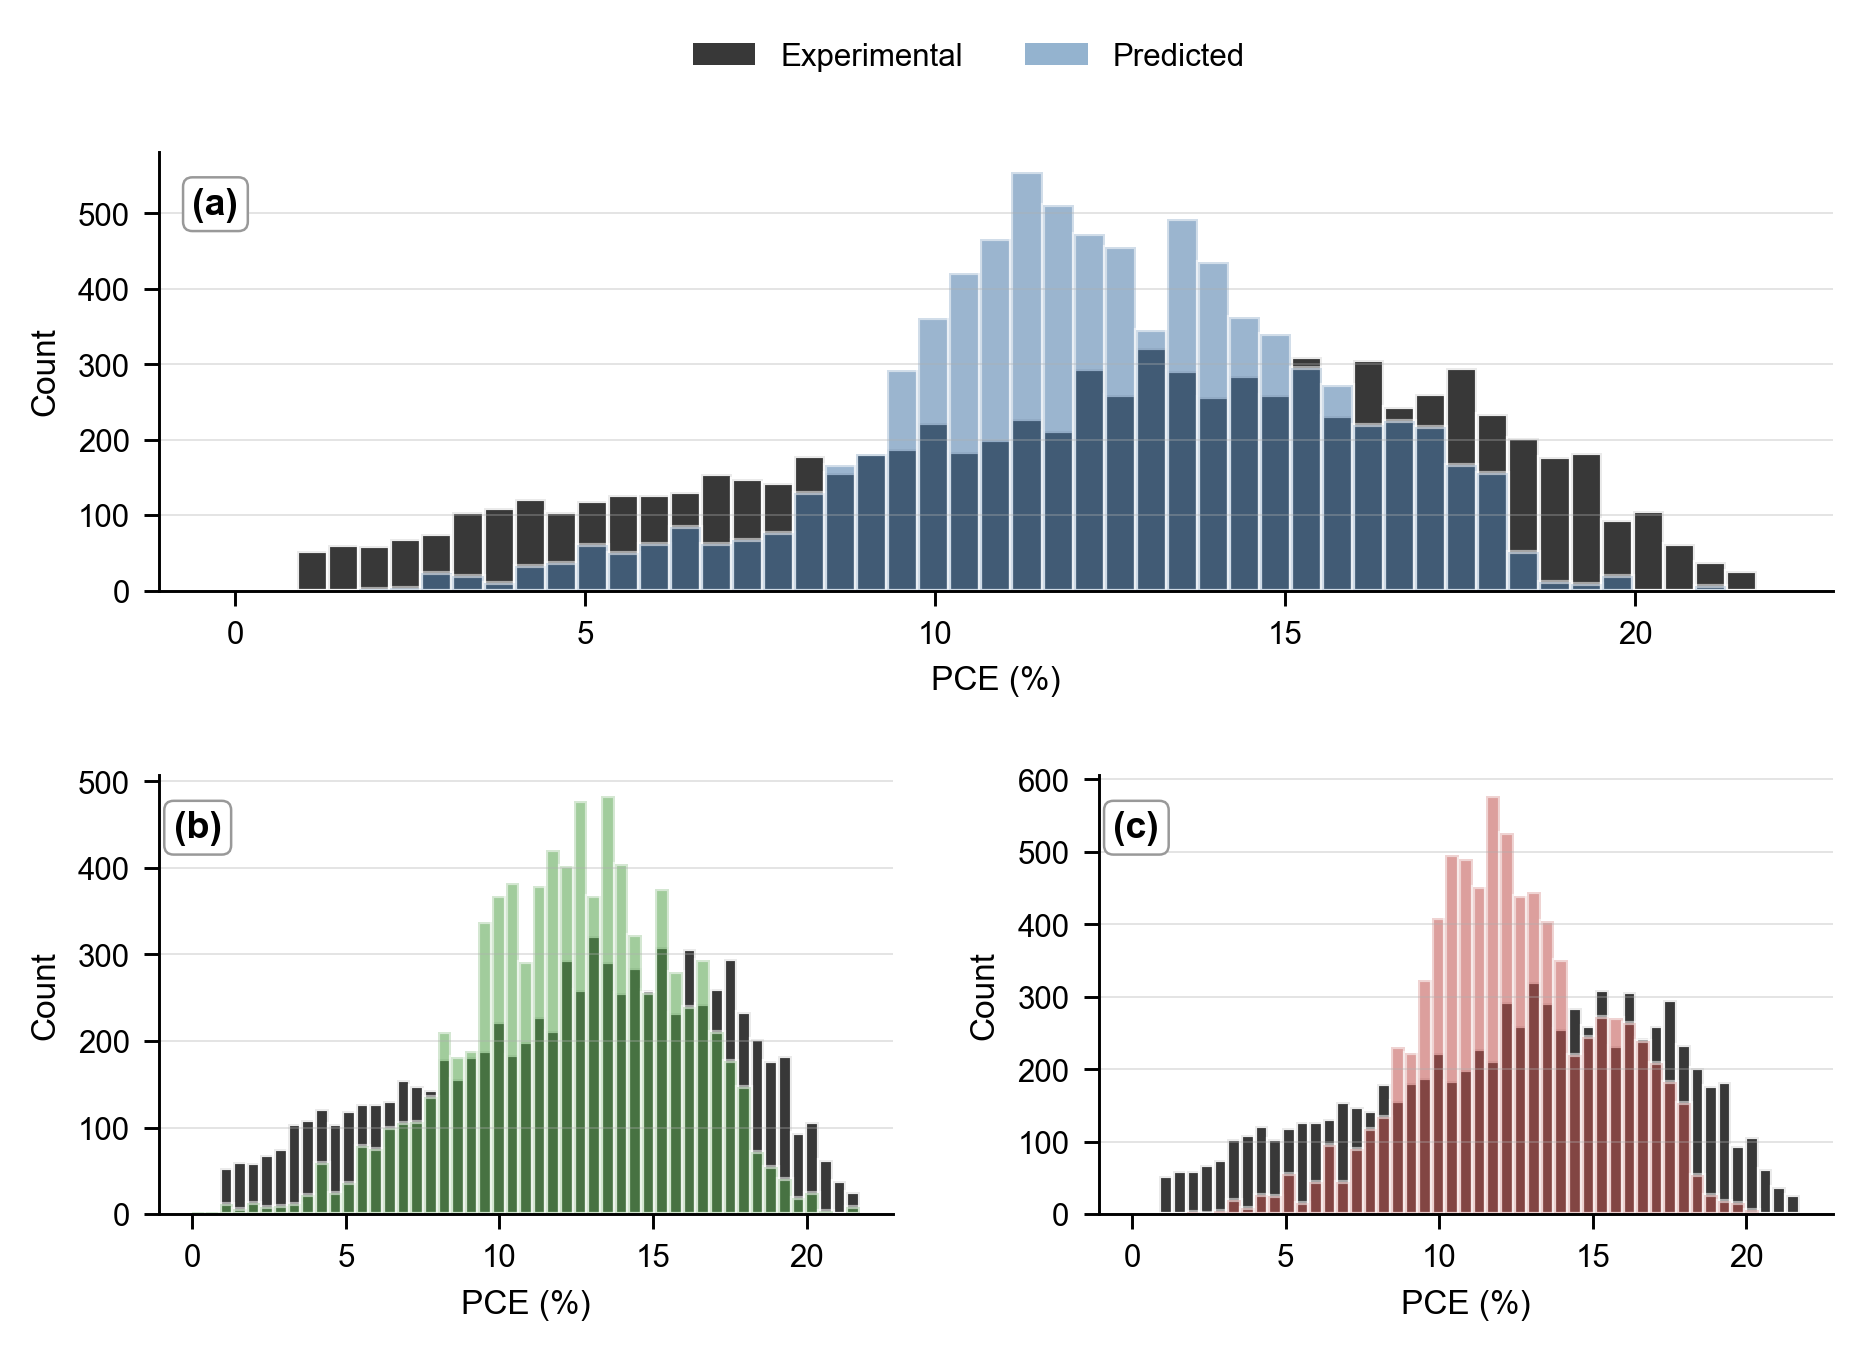
\includegraphics[width=\textwidth]{figures/fig_pce_dist_trio.png}
    \caption{Distribution of experimental and predicted PCE on the first DOI-grouped split (pooled, $t_3^{\mathrm{orig}}$) for (a) CatBoost, (b) the early-stopped MLP and (c) the subsample Gaussian process. Axes extend to the 99.5th percentile of experimental PCE; 272 of the 8,224 test records reach 20\% or more.}
    \label{fig:dist_trio}
\end{figure}

\begin{figure}[t]
    \centering
    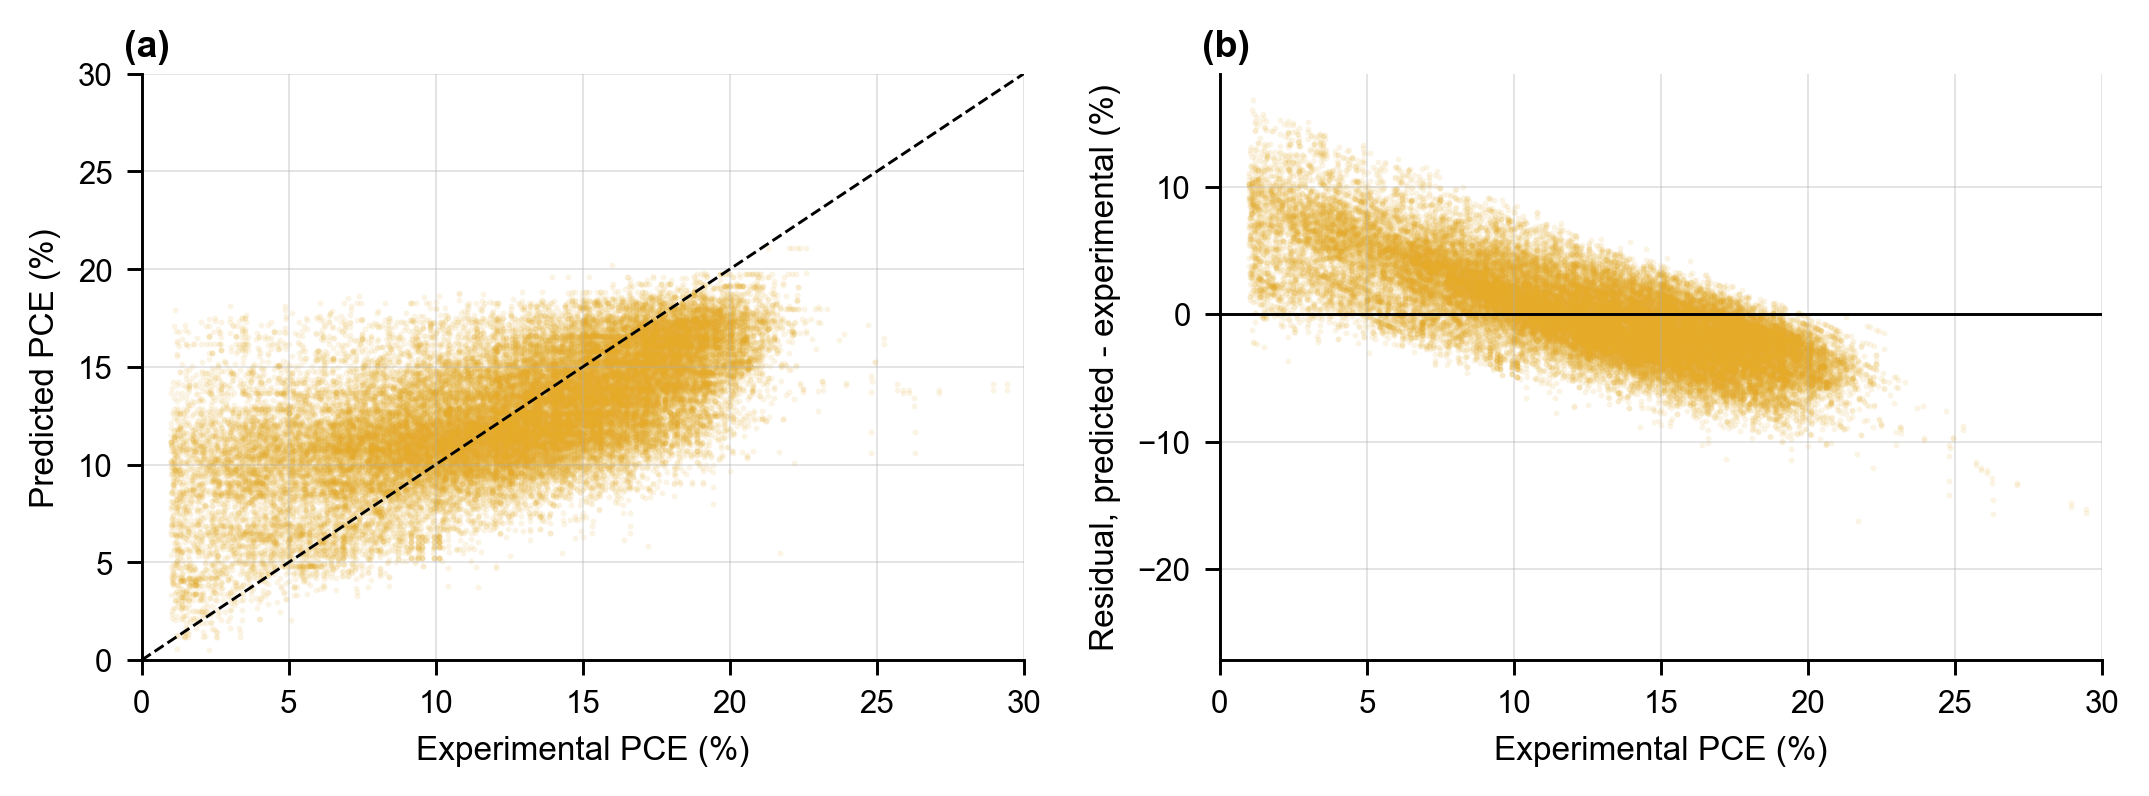
\includegraphics[width=\textwidth]{figures/fig_oof_diagnostics.png}
    \caption{Matched CatBoost ($t_3^{\mathrm{orig}}$, pooled): (a) parity and (b) residuals for the test records of the five DOI-grouped splits stacked (42,142 predictions; records may recur across splits because test sets overlap). The dashed line is $y=x$.}
    \label{fig:parity}
\end{figure}

\subsection{Effect of the evaluation protocol}
\label{sec:splits}

The evaluation protocol had a large influence on measured performance. Table~\ref{tab:split} and Fig.~\ref{fig:split} compare record-level random splitting with DOI-grouped splitting across the feature tiers with identical features, preprocessing, model configurations, filtering and training budgets; only the unit that is split differs. For matched CatBoost the pooled $R^2$ was 0.587, 0.618 and 0.627 under record-level splitting for $t_1$, $t_2$ and $t_3^{\mathrm{orig}}$, compared with 0.368, 0.408 and 0.407 under DOI-grouped splitting, a difference of 0.219, 0.210 and 0.221. MAE rose from 2.20--2.34 to 2.95--3.08 percentage points. The gap is therefore similar for all three tiers.  The record-level fits needed 7,200--11,700 iterations (DOI-grouped fits stop before 500), and the gap was 0.005--0.007 smaller when the cap was 6,000 iterations, so it is sensitive to training length but not to the cap once converged.

\begin{table}[t]
    \centering\small
    \caption{Record-level random versus DOI-grouped splitting for the pooled dataset (mean $\pm$ s.d. over five splits with 20\% of records or publications held out; MAE in PCE percentage points). Features, preprocessing, model configuration and filtering are identical under both protocols; the gap is the mean per-split difference in $R^2$.}
    \label{tab:split}
    \begin{tabular}{llccccc}
        \toprule
        Model & Feature tier & $R^2$ random & $R^2$ DOI-grouped & Gap & MAE rand. & MAE DOI \\
        \midrule
        CatBoost & Database only ($t_1$) & $0.587 \pm 0.009$ & $0.368 \pm 0.024$ & $0.219$ & $2.34$ & $3.08$ \\
        CatBoost & + material ($t_2$) & $0.618 \pm 0.006$ & $0.408 \pm 0.032$ & $0.210$ & $2.23$ & $2.95$ \\
        CatBoost & + material + orig.\ lit.\ ($t_3^{\mathrm{orig}}$) & $0.627 \pm 0.006$ & $0.407 \pm 0.031$ & $0.221$ & $2.20$ & $2.96$ \\
        \midrule
        Ridge & Database only ($t_1$) & $0.363 \pm 0.008$ & $0.307 \pm 0.030$ & $0.056$ & $3.09$ & $3.27$ \\
        Ridge & + material ($t_2$) & $0.408 \pm 0.008$ & $0.354 \pm 0.032$ & $0.055$ & $2.95$ & $3.13$ \\
        Ridge & + material + orig.\ lit.\ ($t_3^{\mathrm{orig}}$) & $0.408 \pm 0.008$ & $0.350 \pm 0.033$ & $0.058$ & $2.95$ & $3.14$ \\
        \bottomrule
    \end{tabular}
\end{table}

\begin{figure}[t]
    \centering
    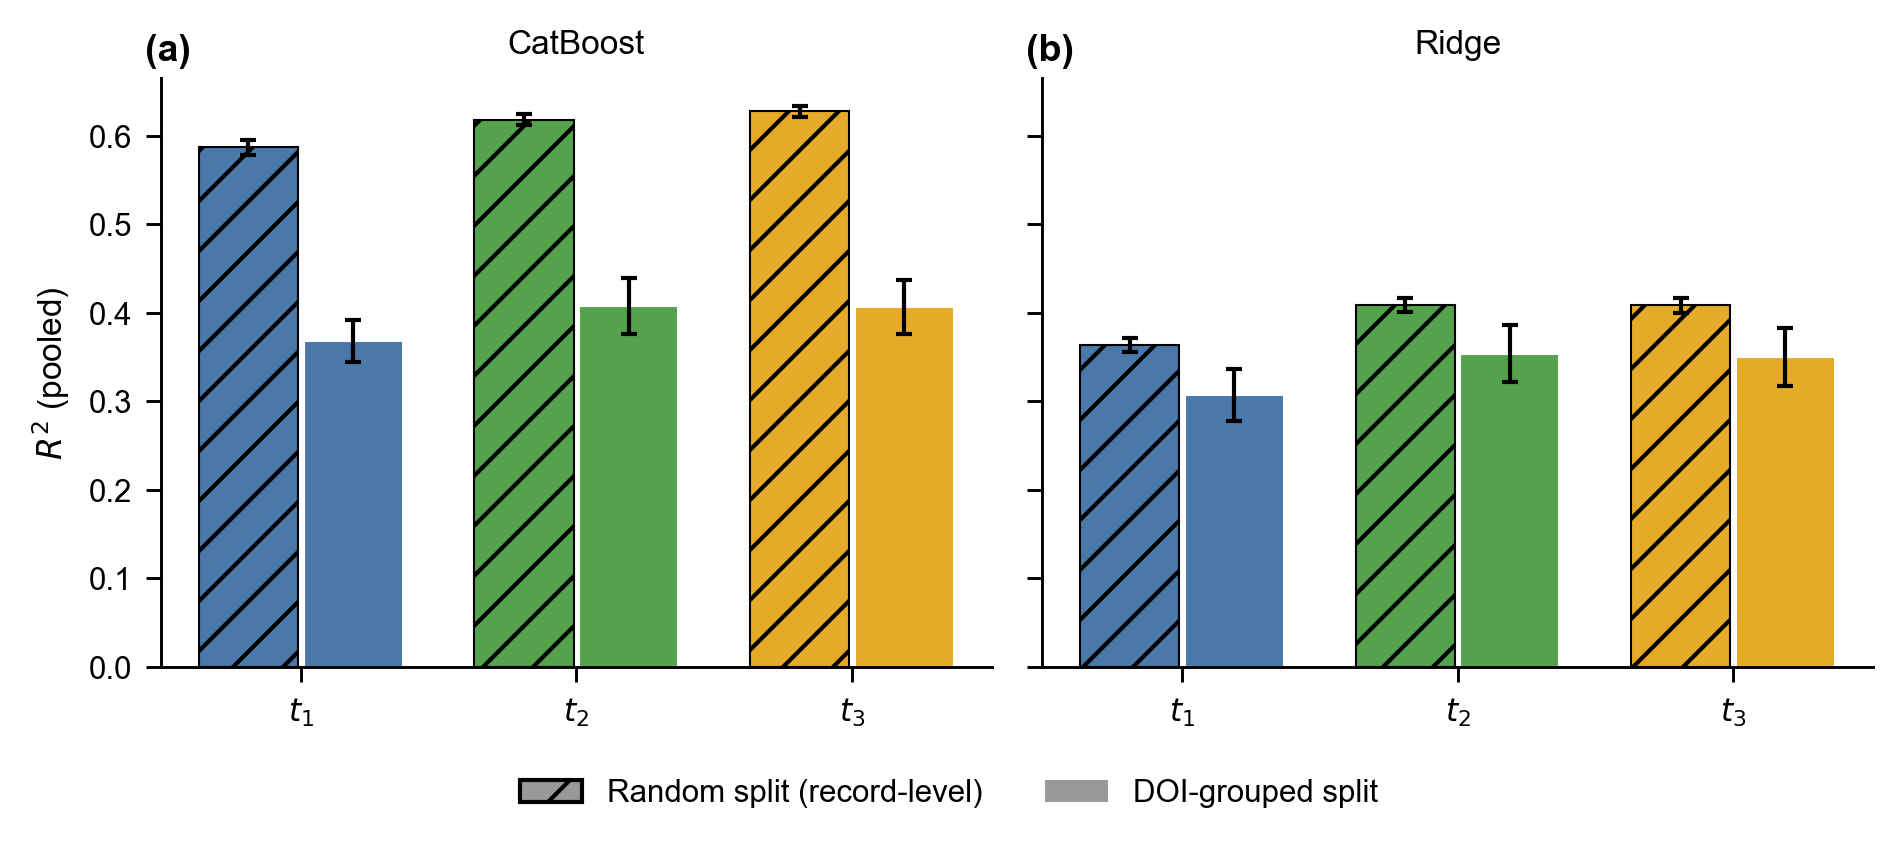
\includegraphics[width=0.7\textwidth]{figures/fig_split_effect.png}
    \caption{Record-level random (hatched) versus DOI-grouped (solid) splits for the three feature tiers ($t_3^{\mathrm{orig}}$: original literature block) with (a) CatBoost and (b) ridge regression (pooled dataset; mean $\pm$ s.d. over five splits).}
    \label{fig:split}
\end{figure}

Two properties of the data make a large gap plausible. First, 69\% of the variance of PCE lies between publications (one-way intraclass correlation by DOI, 0.69), with a median of four records per publication. Second, 31,591 of 41,107 records (77\%) share their complete $t_3^{\mathrm{orig}}$ predictor vector with at least one other record, but only 162 of 7,733 such groups span more than one publication, so near-duplicate devices are almost entirely within-publication; their PCE values differ by a median standard deviation of 1.2 points within a group. A flexible model can memorise publication-specific patterns that a random split leaves available at test time. This reading is consistent with the linear model: for the pooled data ridge regression shows a much smaller gap (0.055--0.058), but it is not a clean capacity test, because the ridge gap for the p-i-n subset is large (0.11--0.19) and ridge is also a weaker predictor on all splits; we did not run a matched-capacity control. The comparison quantifies sensitivity of the measured performance to the splitting protocol on this dataset; it does not show that all of the difference is leakage of identical devices, because the two protocols also produce test sets with different publication compositions, and the stricter lead-author and forward-in-time protocols of Section~\ref{sec:strict} show how much of the DOI-grouped score survives (a little under lead-author grouping, about 0.07 $R^2$ less going forward in time); it still does not amount to an external test. DOI-grouped evaluation answers a specific question, namely performance on papers not seen in training. It does not remove similarity between papers from the same laboratory, and it is not a prospective or external validation. Earlier PDP studies report a larger drop on newly registered records (Fukasawa et al.: $R^2$ 0.7177 under an 8:2 split to 0.45 on 294 newer records) \cite{fukasawa2024effectiveness}, which is directionally consistent, although the targets, feature sets, dataset versions and test sets differ and the numbers are not comparable.

\subsection{Stricter validation: laboratory proxy and forward-in-time splits}
\label{sec:strict}

DOI-grouped splitting leaves two obvious routes for residual similarity: papers from the same laboratory and papers close in time. Table~\ref{tab:strict} compares both with DOI-grouped and record-level evaluation (pooled data, all models and tiers matched). Grouping by lead author lowers the CatBoost $t_3^{\mathrm{orig}}$ $R^2$ only slightly, from 0.407 to $0.395 \pm 0.013$ (MAE 2.92), so on this dataset most of the record-level optimism is already removed at the publication level and the same-laboratory effect captured by this coarse proxy is small. Forward-in-time evaluation is clearly stricter: training on earlier and testing on later publications gives $R^2 = 0.335 \pm 0.058$ for $t_3^{\mathrm{orig}}$ (MAE 3.21; individual windows 0.329, 0.396 and 0.279), against $-0.155$ for the training-mean predictor, whose negative $R^2$ reflects a shift of the PCE distribution towards higher efficiencies over time. Ridge regression degrades similarly (0.283). Neither protocol changes the feature conclusions: the material-property step is $+0.030$ (lead-author) and $+0.052$ (forward in time) in $R^2$, whereas the literature step is $+0.001$ and $-0.010$, i.e.\ absent or negative (per-window values in Table~\ref{tab:temporal}). The temporal result is based on three windows of one dataset snapshot and a partly overlapping training history, so its spread should not be over-interpreted; it indicates that the DOI-grouped estimate of about 0.41 is optimistic for prospective use by roughly 0.07 in $R^2$.

\begin{table*}[t]
    \centering\small
    \caption{Pooled $R^2$ (mean $\pm$ s.d. over splits) by validation protocol, model and feature tier, with matched features, preprocessing and model settings. Splits: five repeats (record-level, DOI-grouped, lead-author-grouped) or three forward windows. MAE refers to $t_3^{\mathrm{orig}}$ (percentage points). The pooled record-level CatBoost fits are the converged ones (20,000-iteration cap; Section~\ref{sec:splits}).}
    \label{tab:strict}
    \setlength{\tabcolsep}{4pt}
    \begin{tabular}{llrrcccc}
        \toprule
        Protocol & Model & $N_\mathrm{test}$ & Splits & $t_1$ & $t_2$ & $t_3^{\mathrm{orig}}$ & MAE ($t_3^{\mathrm{orig}}$) \\
        \midrule
        Record-level & CatBoost & 8,222 & 5 & $0.587 \pm 0.009$ & $0.618 \pm 0.006$ & $0.627 \pm 0.006$ & $2.20$ \\
        Record-level & Ridge & 8,222 & 5 & $0.363 \pm 0.008$ & $0.408 \pm 0.008$ & $0.408 \pm 0.008$ & $2.95$ \\
        Record-level & Mean & 8,222 & 5 & $-0.000 \pm 0.000$ & $-0.000 \pm 0.000$ & $-0.000 \pm 0.000$ & $4.06$ \\
        DOI-grouped & CatBoost & 8,428 & 5 & $0.368 \pm 0.024$ & $0.408 \pm 0.032$ & $0.407 \pm 0.031$ & $2.96$ \\
        DOI-grouped & Ridge & 8,428 & 5 & $0.307 \pm 0.030$ & $0.354 \pm 0.032$ & $0.350 \pm 0.033$ & $3.14$ \\
        DOI-grouped & Mean & 8,428 & 5 & $-0.001 \pm 0.001$ & $-0.001 \pm 0.001$ & $-0.001 \pm 0.001$ & $4.08$ \\
        Lead-author-grouped & CatBoost & 8,280 & 5 & $0.363 \pm 0.019$ & $0.394 \pm 0.018$ & $0.395 \pm 0.013$ & $2.92$ \\
        Lead-author-grouped & Ridge & 8,280 & 5 & $0.313 \pm 0.011$ & $0.353 \pm 0.017$ & $0.350 \pm 0.018$ & $3.05$ \\
        Lead-author-grouped & Mean & 8,280 & 5 & $-0.002 \pm 0.002$ & $-0.002 \pm 0.002$ & $-0.002 \pm 0.002$ & $3.98$ \\
        Forward in time & CatBoost & 6,436 & 3 & $0.293 \pm 0.059$ & $0.345 \pm 0.049$ & $0.335 \pm 0.058$ & $3.21$ \\
        Forward in time & Ridge & 6,436 & 3 & $0.227 \pm 0.075$ & $0.286 \pm 0.087$ & $0.283 \pm 0.091$ & $3.34$ \\
        Forward in time & Mean & 6,436 & 3 & $-0.155 \pm 0.027$ & $-0.155 \pm 0.027$ & $-0.155 \pm 0.027$ & $4.57$ \\
        \bottomrule
    \end{tabular}
\end{table*}

\begin{table}[t]
    \centering\small
    \caption{Forward-in-time windows (pooled CatBoost, $R^2$): latest training date, earliest test date, record counts and tier results.}
    \label{tab:temporal}
    \setlength{\tabcolsep}{2pt}\footnotesize
    \begin{tabular}{rllrrrrr}
        \toprule
        Win. & Train until & Test from & $n_\mathrm{train}$ & $n_\mathrm{test}$ & $t_1$ & $t_2$ & $t_3^{\mathrm{orig}}$ \\
        \midrule
        1 & 2017-12-26 & 2018-05-02 & 18,529 & 6,502 & $0.284$ & $0.335$ & $0.329$ \\
        2 & 2018-07-20 & 2018-12-12 & 24,074 & 6,322 & $0.356$ & $0.398$ & $0.396$ \\
        3 & 2019-01-27 & 2019-07-19 & 29,429 & 6,484 & $0.240$ & $0.302$ & $0.279$ \\
        \bottomrule
    \end{tabular}
\end{table}

\subsection{Contribution of material-property and literature-derived features}
\label{sec:features}

\subsubsection{Material-property descriptors.}
Adding material-property descriptors ($t_1 \rightarrow t_2$) increased $R^2$ by 0.040 (pooled), 0.047 (p-i-n) and 0.029 (n-i-p) and lowered RMSE by 0.125, 0.130 and 0.093 percentage points (Table~\ref{tab:delta}). The pooled gain had a cluster-bootstrap interval excluding zero in all five splits (two of five for p-i-n and three of five for n-i-p, which have fewer test publications), and $R^2$ improved in all 15 split--subset pairs. Because $t_1$ contains no explicit transport-layer material identities (Section~\ref{sec:integration}), the $t_2$ descriptors convey both which materials were used and their reference properties; each property is a fixed function of the material, so this gain could reflect knowledge of which materials were used rather than their property values. A material-identity control separates the two. Adding only the ETL, HTL and perovskite identities to $t_1$ as native CatBoost categorical features (disjoint DOI-grouped five-fold, three seeds, same CatBoost configuration, 41,107 records) gives $R^2 = 0.406$, against 0.370 for $t_1$ and 0.407 for $t_2$; the 102 descriptor columns add $+0.001$ over identity alone (interval for the paired MSE difference includes zero), and descriptors on top of identity add $+0.004$ (also not distinguishable from zero). The gain of $t_2$ over $t_1$ is therefore attributable to knowing which transport and absorber materials a device contains, not to the physical descriptor values; transferable physical information is not demonstrated by this comparison (a leave-material-out test would be needed). This is consistent with prior work showing that the representation of material and process information strongly affects PCE prediction \cite{fukasawa2024effectiveness}, and it shows that the benefit persists when entire publications are held out.

\subsubsection{Original LLM-derived literature block.}
Adding the original block of 44 LLM-derived literature predictors ($t_2 \rightarrow t_3^{\mathrm{orig}}$) under the same configuration produced no measurable change: $\Delta R^2$ was $-0.001$ (pooled), $+0.002$ (p-i-n) and $+0.001$ (n-i-p), $t_3^{\mathrm{orig}}$ was better than $t_2$ in $R^2$ in only 1, 3 and 3 of five splits, and in none of the 15 split--subset pairs did the bootstrap interval for the paired difference exclude zero (Table~\ref{tab:delta}). The controls in Table~\ref{tab:groups} point the same way: adding the literature block to the database tier without material properties gives $R^2 = 0.372 \pm 0.026$ against 0.368 for $t_1$; removing the two reporting-completeness flags from $t_3^{\mathrm{orig}}$ leaves $R^2$ unchanged (0.407); and appending 32 columns of pure noise to $t_2$ changes $R^2$ by $-0.004$ (0.404 against 0.408), i.e.\ by about as much as the literature block does. The literature features are available for 36.2\% of records, are defined per publication, and are largely redundant with PDP columns that $t_1$ already contains (Section~\ref{sec:extraction}: exact agreement in most records, new information in about 1--5\% of records), which is a plausible reason for the null result; we conclude that this block adds no detectable predictive information beyond the database and material tiers for unseen publications. It motivated the more targeted recipe-flag representation evaluated in Section~\ref{sec:recipe_results}. Under record-level splitting the same comparison gives $R^2$ 0.618 versus 0.627 ($+0.009$), again small, so publication-constant features are not the main source of the random-split advantage here.

\subsubsection{Recipe-flag features on reserved publications.}
\label{sec:recipe_results}
The recipe-flag block $t_3$ (Section~\ref{sec:recipe}) was developed on development publications only. There, the remaining content of the extraction JSON (token bags, numeric quantities, device-matched layer values, gap-filling of PDP fields) added at most about $+0.004$ $R^2$, and giving $t_2$ the PDP's own curated process columns for the same papers added only $+0.022$, which motivated a block of recipe identities. On covered development publications the flags gave $+0.007$ $R^2$ (12 of 15 folds), five DOI-permuted copies gave $-0.009$ to $+0.002$, dropping any one flag group reduced the gain, and no single group reproduced it, so the signal is distributed and close to the noise floor. A role-scoped variant of the flags gave $+0.001$, so differences between variants are within development noise.

The reserved publications were then scored once (Table~\ref{tab:v4}, Fig.~\ref{fig:v4}). Under the same default settings, adding the flags to $t_2$ changed $R^2$ by $+0.0071$ (95\% interval $-0.0007$ to $+0.0157$; positive in 4 of 5 seeds) on the 5,460 covered records and by $+0.0025$ ($-0.0011$ to $+0.0062$; 4 of 5 seeds) on all 14,125 reserved records. When each tier used its own tuned configuration, covered-record $R^2$ was 0.361 for $t_2$ and 0.371 for $t_3$ ($\Delta R^2 = +0.0094$, $-0.0016$ to $+0.0219$; 5 of 5 seeds), and on all records both tiers reached about 0.41 ($\Delta R^2 = +0.0015$, $-0.0039$ to $+0.0067$; 3 of 5 seeds). The direction therefore agrees with the development result, and in point estimate the flags exceed all five permuted-block controls (covered $-0.0049$ to $+0.0015$; all records $-0.0028$ to $+0.0007$) and a coverage-indicator-only control ($+0.0015$ and $+0.0011$). Every interval, however, includes zero. We read these results as a small, suggestive improvement that is concentrated where the information exists, not as an established gain in generalisation.

Four features of the evidence limit how far it can be pushed. First, the size of the effect depends on the estimator: with $t_2$'s tuned configuration used for both tiers the covered $\Delta R^2$ falls to $+0.0024$ ($-0.0077$ to $+0.0131$) and the all-record difference is $-0.0016$. Second, tuning alone moves $t_2$ by $+0.0020$ (covered) to $+0.0030$ (all records), comparable to the flag effect, so the tuned comparison should not be read as a feature gain by itself. Third, the flag block was chosen after development comparisons, and the reserved publications, though not used for any choice in this representation, were examined in earlier experiments with other feature sets. Fourth, a single reserved split of about 1,000 covered publications resolves $R^2$ differences only to roughly $\pm 0.01$. The flags are also available for only 36.6\% of records, which dilutes any benefit on the full data; a larger signal would require full-text extraction for the roughly 4,500 publications that currently lack it, which we did not do. These results use a different partition and, for the tuned arms, different configurations from the controlled ablation and from Table~\ref{tab:dev}, so they must not be combined with those tables.

\begin{table}[ht]
    \centering\small
    \caption{Recipe-flag block on reserved publications ($t_3$ versus $t_2$; one reserved partition, trained on development publications; $\Delta R^2$ is $t_3$ minus $t_2$ with a 95\% publication-cluster bootstrap interval; ``Seeds $>0$'' counts the five seed-level differences). \emph{Default}: matched default CatBoost configuration for both tiers; \emph{each tuned}: each tier's own selected configuration; \emph{$t_3^{\mathrm{orig}}$'s} and \emph{$t_2$'s} tuned configuration: that configuration applied to both tiers. Covered: 5,460 records from 1,005 publications with extraction data; all: 14,125 records from 2,619 publications. This protocol differs from Tables~\ref{tab:tiers} and~\ref{tab:dev}.}
    \label{tab:v4}
    \begin{tabular}{llccccc}
        \toprule
        Records & Settings & $R^2$ ($t_2$) & $R^2$ ($t_3$) & $\Delta R^2$ & 95\% interval & Seeds $>0$ \\
        \midrule
        Covered & Default & 0.359 & 0.366 & $+0.0071$ & $[-0.0007, +0.0157]$ & 4/5 \\
        Covered & Each tuned & 0.361 & 0.371 & $+0.0094$ & $[-0.0016, +0.0219]$ & 5/5 \\
        Covered & $t_3^{\mathrm{orig}}$'s tuned config. & 0.364 & 0.371 & $+0.0066$ & $[-0.0021, +0.0162]$ & 4/5 \\
        Covered & $t_2$'s tuned config. & 0.361 & 0.364 & $+0.0024$ & $[-0.0077, +0.0131]$ & 3/5 \\
        \midrule
        All & Default & 0.403 & 0.406 & $+0.0025$ & $[-0.0011, +0.0062]$ & 4/5 \\
        All & Each tuned & 0.406 & 0.408 & $+0.0015$ & $[-0.0039, +0.0067]$ & 3/5 \\
        All & $t_3^{\mathrm{orig}}$'s tuned config. & 0.405 & 0.408 & $+0.0026$ & $[-0.0015, +0.0067]$ & 2/5 \\
        All & $t_2$'s tuned config. & 0.406 & 0.405 & $-0.0016$ & $[-0.0064, +0.0030]$ & 2/5 \\
        \bottomrule
    \end{tabular}
\end{table}

\begin{figure}[t]
    \centering
    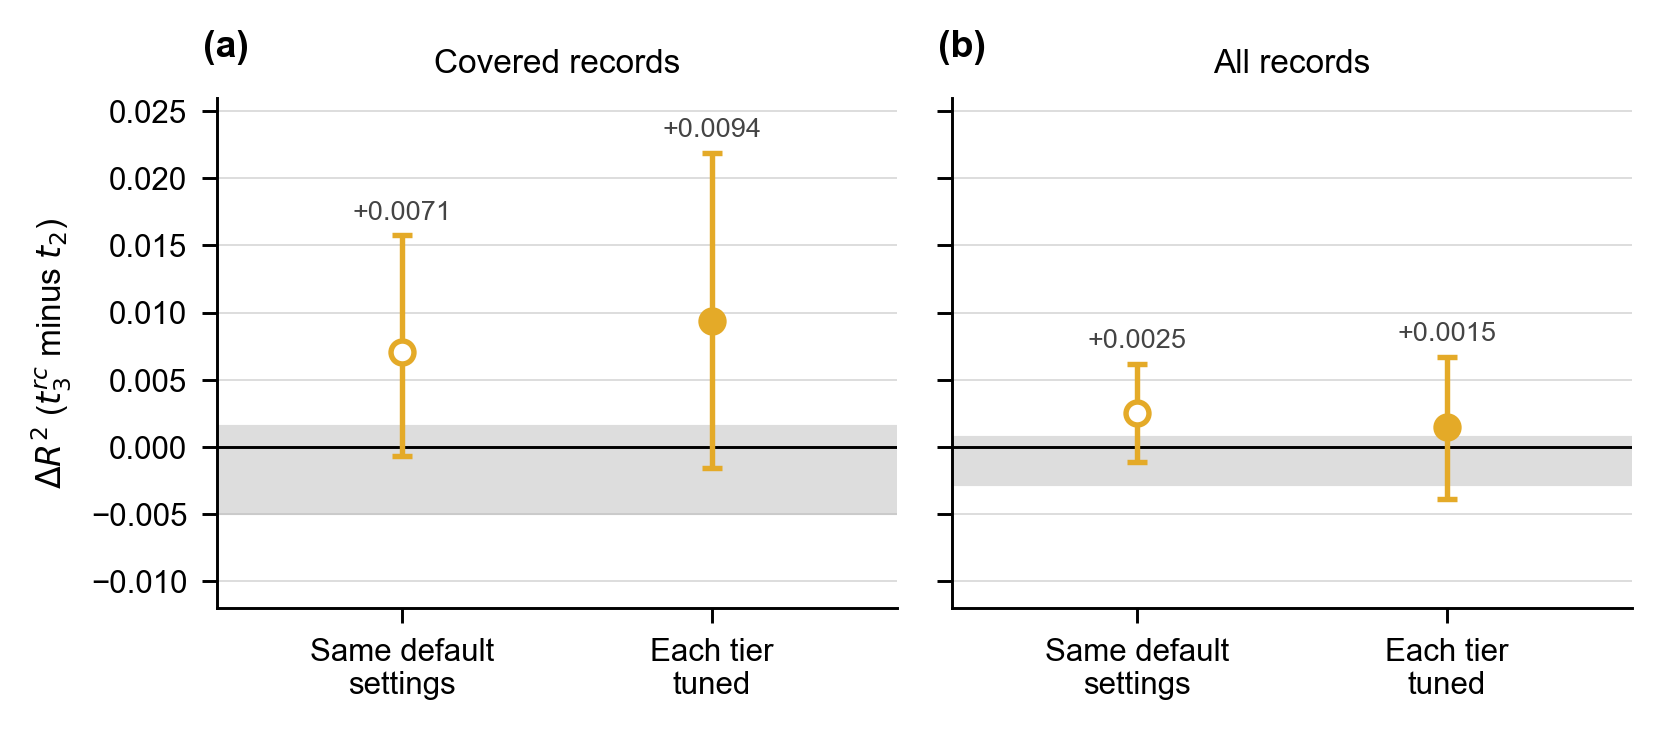
\includegraphics[width=0.8\textwidth]{figures/fig_v4_recipe.png}
    \caption{Effect of the recipe-flag block on reserved publications: $\Delta R^2$ ($t_3$ minus $t_2$) with 95\% publication-cluster bootstrap intervals for (a) covered records and (b) all records, under the same default settings (open symbols) and with each tier separately tuned (filled symbols). Grey bands mark the range of five DOI-permuted-block controls under default settings. All intervals include zero.}
    \label{fig:v4}
\end{figure}

\begin{table}[t]
    \centering\small
    \caption{Paired differences between tiers (matched CatBoost, DOI-grouped splits). $\Delta R^2$ and $\Delta$RMSE are means over the five splits; ``better'' is the number of splits in which $R^2$ improved; ``CI$\neq0$'' is the number of splits in which the 95\% DOI-cluster bootstrap interval of the paired $\Delta R^2$ excludes zero. Test sets overlap across splits, so no pooled significance test is reported.}
    \label{tab:delta}
    \begin{tabular}{lcccccccc}
        \toprule
        & \multicolumn{4}{c}{$t_1\!\to\! t_2$} & \multicolumn{4}{c}{$t_2\!\to\! t_3^{\mathrm{orig}}$} \\
        \cmidrule(lr){2-5}\cmidrule(lr){6-9}
        Subset & $\Delta R^2$ & $\Delta$RMSE & better & CI$\neq0$ & $\Delta R^2$ & $\Delta$RMSE & better & CI$\neq0$ \\
        \midrule
        Pooled & $+0.040$ & $-0.125$ & 5/5 & 5/5 & $-0.001$ & $+0.004$ & 1/5 & 0/5 \\
        p-i-n & $+0.047$ & $-0.130$ & 5/5 & 2/5 & $+0.002$ & $-0.008$ & 3/5 & 0/5 \\
        n-i-p & $+0.029$ & $-0.093$ & 5/5 & 3/5 & $+0.001$ & $-0.005$ & 3/5 & 0/5 \\
        \bottomrule
    \end{tabular}
\end{table}

\begin{table}[t]
    \centering\small
    \caption{Feature-group controls (matched CatBoost, DOI-grouped splits; mean $\pm$ s.d. over five splits). Compare with Table~\ref{tab:tiers}.}
    \label{tab:groups}
    \begin{tabular}{llcccc}
        \toprule
        Subset & Variant & Feat. & $R^2$ & MAE & RMSE \\
        \midrule
        Pooled & $t_1$ + LLM (no material) & 121 & $0.372 \pm 0.026$ & $3.060 \pm 0.053$ & $3.895 \pm 0.061$ \\
        Pooled & $t_3^{\mathrm{orig}}$ minus 2 completeness flags & 219 & $0.407 \pm 0.028$ & $2.953 \pm 0.075$ & $3.787 \pm 0.078$ \\
        Pooled & $t_2$ + 32 noise columns & 211 & $0.404 \pm 0.029$ & $2.970 \pm 0.065$ & $3.796 \pm 0.076$ \\
        p-i-n & $t_1$ + LLM (no material) & 122 & $0.251 \pm 0.071$ & $3.150 \pm 0.058$ & $4.065 \pm 0.136$ \\
        p-i-n & $t_3^{\mathrm{orig}}$ minus 2 completeness flags & 220 & $0.292 \pm 0.070$ & $3.052 \pm 0.061$ & $3.951 \pm 0.134$ \\
        p-i-n & $t_2$ + 32 noise columns & 211 & $0.288 \pm 0.072$ & $3.067 \pm 0.063$ & $3.962 \pm 0.144$ \\
        n-i-p & $t_1$ + LLM (no material) & 120 & $0.378 \pm 0.014$ & $3.050 \pm 0.038$ & $3.907 \pm 0.053$ \\
        n-i-p & $t_3^{\mathrm{orig}}$ minus 2 completeness flags & 218 & $0.407 \pm 0.012$ & $2.960 \pm 0.024$ & $3.816 \pm 0.051$ \\
        n-i-p & $t_2$ + 32 noise columns & 210 & $0.402 \pm 0.009$ & $2.976 \pm 0.025$ & $3.830 \pm 0.053$ \\
        \bottomrule
    \end{tabular}
\end{table}

\subsection{Interpretation of model predictions}
\label{sec:shap}

\subsubsection{Global importance.}
SHAP values are attributions for the fitted model and do not demonstrate predictive benefit or causal effects. Perovskite quenching/crystallisation was the highest-ranked predictor in all three models (mean $|$SHAP$|$ 0.727, 0.525 and 1.002 PCE percentage points for the pooled, p-i-n and n-i-p models; Fig.~\ref{fig:beeswarm}). It is the PDP binary field \texttt{Perovskite\_deposition\_quenching\_induced\_crystallisation} (1 if a quenching-induced crystallisation step was reported, 0 if not; 20,657 and 22,731 records of the PDP export, 10 missing). In the pooled model the next features were total ion count (0.265), the missingness indicator of the perovskite photoluminescence maximum (0.229), HTL deposition method (0.212), perovskite annealing time (0.202), average perovskite atomic mass (0.197), average perovskite radius (0.192) and HTL band gap (0.186). In the p-i-n model HTL band gap ranked second (0.506) and ETL deposition method third (0.410). Because material properties are fixed functions of material identity, layer-property features such as HTL band gap also act as identifiers of the material used in that layer. Aggregating importance by feature group (Fig.~\ref{fig:groups}) shows that material-property (33--38\%) and process (36--42\%) variables dominate, followed by composition (13--15\%) and device (6--8\%) descriptors.

The 44 predictors of the original literature block account for 4.0\% (pooled), 3.9\% (p-i-n) and 3.6\% (n-i-p) of the total absolute SHAP attribution, showing that the fitted models use them, although the ablation above shows that this use does not translate into held-out benefit. The highest-ranked literature feature in all three models was \texttt{json\_numeric\_values\_found}, the number of numerical values recovered from a paper (rank 35, 40 and 28 in the pooled, p-i-n and n-i-p models), which reflects how completely a publication reports its experimental details rather than a material or processing parameter. One possible explanation, which we did not test, is that publication-constant features can be used to separate training publications without carrying information that transfers to unseen ones.

\begin{figure}[t]
    \centering
    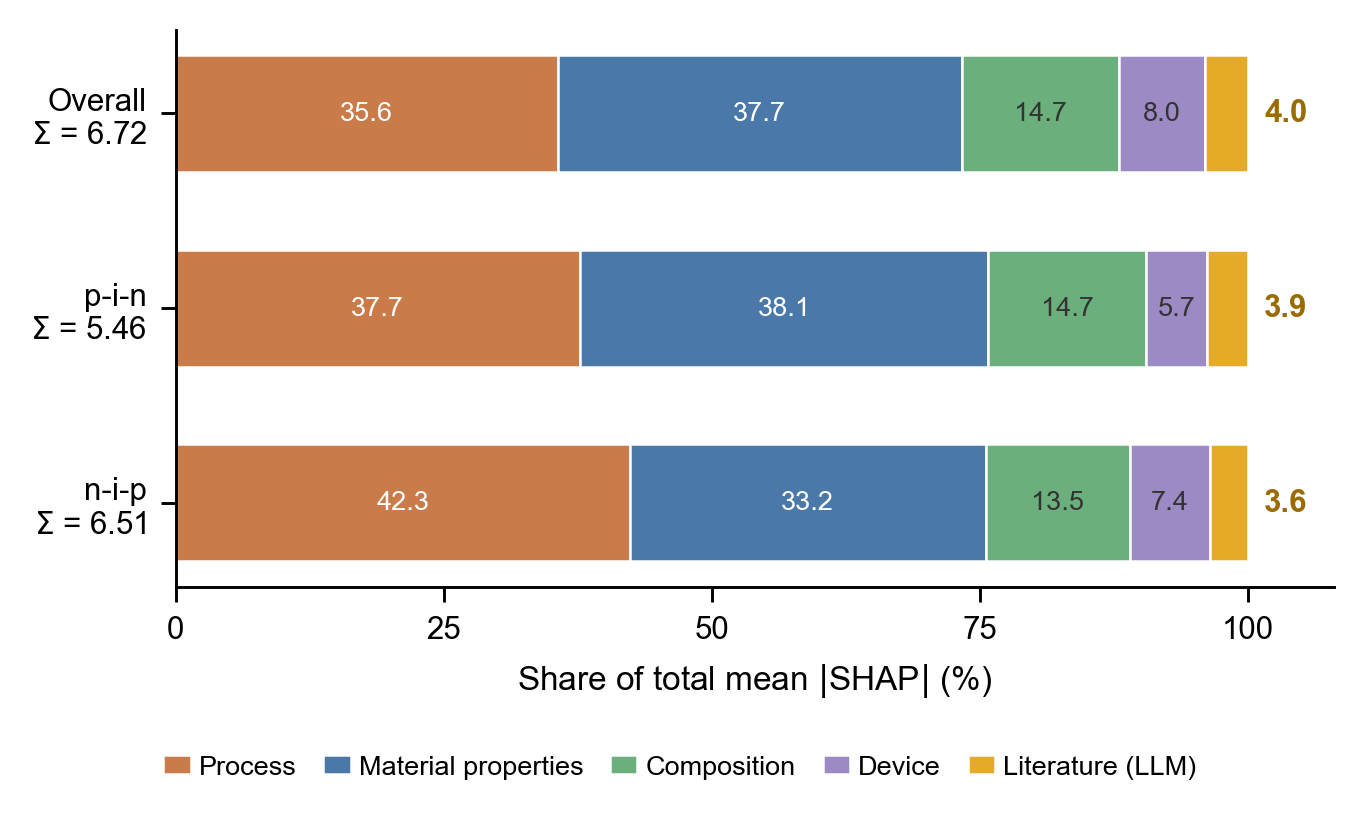
\includegraphics[width=\textwidth]{figures/fig_shap_groups.png}
    \caption{Share of total feature attribution by feature group for the matched $t_3^{\mathrm{orig}}$ CatBoost models on the first DOI-grouped split (1,500 test records). Bars are group-summed mean $|$SHAP$|$ as a fraction of the model total (6.72 pooled, 5.46 p-i-n, 6.51 n-i-p PCE points; 223 features per model). Attribution is not predictive benefit.}
    \label{fig:groups}
\end{figure}

\subsubsection{Architecture-specific associations.}
For p-i-n devices the highest-ranked features were quenching/crystallisation (0.525), HTL band gap (0.506), ETL deposition method (0.410), perovskite thickness (0.234), HTL LUMO (0.229) and Pb fraction (0.168). For n-i-p devices, quenching/crystallisation (1.002) was followed by HTL deposition method (0.303), average perovskite radius (0.285), average perovskite atomic mass (0.220), ETL deposition method (0.202) and perovskite deposition method (0.195). Because the two models were fitted to different records, these differences describe learned associations, not differences in physical effects between architectures.

\begin{figure}[t]
    \centering
    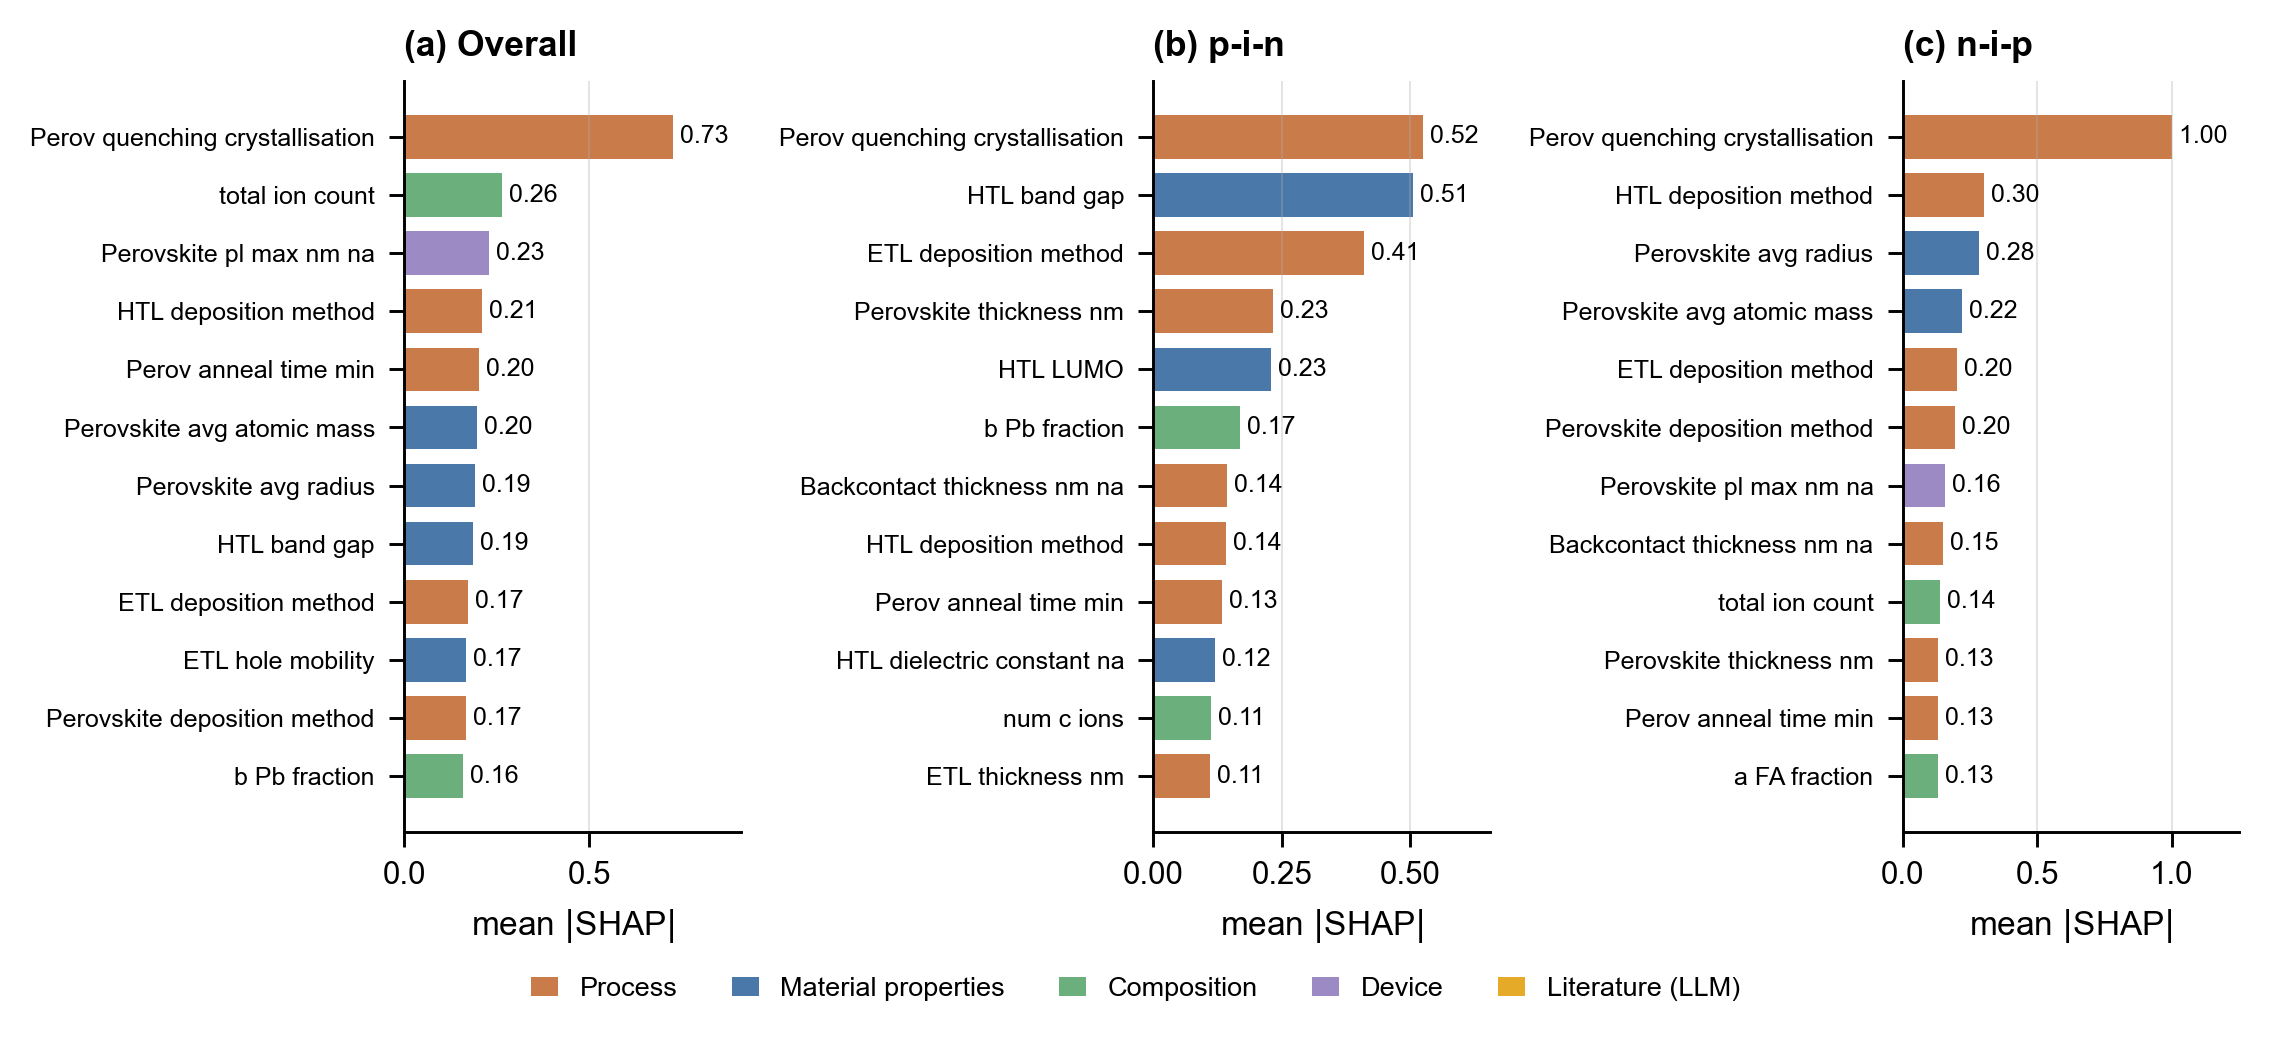
\includegraphics[width=\textwidth]{figures/shap.png}
    \caption{Twelve highest-ranked features by mean $|$SHAP$|$ for the (a) pooled, (b) p-i-n and (c) n-i-p matched $t_3^{\mathrm{orig}}$ CatBoost models (first DOI-grouped split). Bar colour denotes feature group (as in Fig.~\ref{fig:groups}); values and the horizontal axes are mean $|$SHAP$|$ in PCE percentage points; the models use the original literature block; \texttt{na} denotes a missingness indicator.}
    \label{fig:beeswarm}
\end{figure}

\subsection{Comparison with previous PDP-based studies}

Table~\ref{tab:previous_pdp_studies} summarises what the two most closely related PDP studies did and reported. The numbers are not comparable with ours: Roberts et al.\ predict short-circuit current density ($J_{\mathrm{SC}}$, RMSE in mA\,cm$^{-2}$), whereas we predict PCE (errors in percentage points), and the record sets, feature sets and test sets also differ. The Fukasawa et al.\ entries are left to be completed. As an indirect, like-for-like reference we ran the \emph{settings} associated with these studies inside our framework (Table~\ref{tab:baselines}): XGBoost with library defaults (the setting of Roberts-style pipelines) and a random forest (the best model of Fukasawa et al.) on the database-only tier $t_1$, evaluated on the same DOI-grouped splits. They reach $R^2 = 0.334$ and 0.295, against 0.368 for matched CatBoost on $t_1$. These are not re-implementations of the original feature engineering (one-hot layered encodings and duplicate averaging for Roberts et al.; Oliynyk composition vectors and zero complement for Fukasawa et al.), and we did not re-run the original pipelines.

\begin{table}[t]
    \centering
    \small
    \caption{Related PDP-based studies as described in the cited articles, and this study. Targets differ: Roberts et al.\ predict $J_{\mathrm{SC}}$ (RMSE in mA\,cm$^{-2}$) and this study predicts PCE (MAE in percentage points), so their absolute metrics are not directly comparable. The two rows for this study are different evaluations (a controlled five-split ablation with a fixed configuration and the original literature block, and a single reserved-publication set scored with tuned CatBoost and the recipe-flag block) and should not be mixed.}
    \label{tab:previous_pdp_studies}
    \begin{tabular}{p{2.7cm}p{1.2cm}p{3.7cm}p{4.6cm}}
        \toprule
        Study & Target & Partitioning & Model and reported performance \\
        \midrule
        Roberts et al.\ \cite{roberts2024machine} & $J_{\mathrm{SC}}$ & 80/10/10 train/validation/test; duplicates averaged & XGBoost: $R^2 = 0.35$, RMSE $= 3.58$ mA\,cm$^{-2}$ \\
        Fukasawa et al.\ \cite{fukasawa2024effectiveness} & -- & -- & -- \\
        This study, controlled ablation & PCE & DOI-grouped repeated holdout (five splits), DOI-disjoint validation & Matched CatBoost, pooled, original-block $t_3^{\mathrm{orig}}$: $R^2 = 0.407 \pm 0.031$, MAE $= 2.96 \pm 0.08$ \\
        This study, reserved publications & PCE & DOI-grouped holdout (2,619 reserved publications), DOI-disjoint validation & Tuned CatBoost, all 14,125 records, $t_3$: $R^2 = 0.408$, MAE $= 2.94$ \\
        \bottomrule
    \end{tabular}
\end{table}

\subsection{Limitations}
Results come from a single database with heterogeneous reporting, and 69\% of the PCE variance lies between publications, so held-out $R^2$ values near 0.4 mean that most between-paper variation is not explained by the available descriptors. The DOI-grouped holdout measures generalization to unseen publications, but the five repeated test sets overlap, so the reported spreads are not those of an independent repeated grouped cross-validation, and the cluster-bootstrap intervals address within-test dependence only. Grouping by DOI does not separate publications from the same research group, which may share materials and recipes across papers; grouping by lead-author surname is only a coarse laboratory proxy, and the forward-in-time evaluation (three windows, Section~\ref{sec:strict}) lowers $R^2$ to about 0.33; neither is an external validation on independently collected devices. The 232 records without a DOI were kept together, which is conservative but not informative about their true publications. Some publications report the same device configuration (1,277 records in 162 groups of identical predictor vectors span more than one DOI), and such cross-publication near-duplicates can still fall on both sides of a DOI-grouped split. LLM-derived features were available for about 37\% of the records (36.2\% for the original block, 36.6\% for the recipe flags), extraction accuracy was assessed only against a second curated source and not against a hand-annotated gold set, and the literature features are defined per publication and therefore cannot distinguish between devices within the same paper. The recipe-flag evidence rests on one reserved partition of about 1,000 covered publications (resolution roughly $\pm 0.01$ $R^2$), the flag block was chosen after development comparisons, the reserved publications had been examined in earlier experiments with other feature representations, and the apparent gain depends on the CatBoost configuration. The controlled ablation, the model-development table, the SHAP analysis and the protocol comparisons use the original literature block, not the recipe flags, and no five-split ablation of the recipe flags was run. Material-property descriptors are material-level reference values, so they identify materials as much as they describe them. The reference Gaussian process was fitted to a subsample and the MLP was not extensively tuned, so Table~\ref{tab:baselines} does not rank model families. Predictions saturate near 21\% PCE, under-predict high-efficiency devices, can be negative, and devices with reported PCE below 1\% were excluded.


% ---------------- CONCLUSION ----------------
\section{Conclusion}
We built and audited a PCE prediction pipeline for the Perovskite Database Project and evaluated it on unseen publications with DOI-grouped, validation-based holdouts. Two findings are supported by the evidence. First, performance on unseen publications is moderate: a fixed CatBoost model reached a pooled $R^2$ of 0.407 (MAE 2.96 percentage points) and a validation-tuned ensemble 0.418 (MAE 2.92), with substantial architecture dependence (n-i-p 0.41, p-i-n 0.30) and a split-to-split standard deviation of about 0.03; simple ridge regression and a properly trained MLP or Gaussian process are within 0.03--0.06 $R^2$. In a controlled, nested comparison, curated material-property descriptors improved $R^2$ by 0.040 (pooled), a gain that adding only the material identities to $t_1$ reproduces ($R^2$ 0.406 versus 0.407), whereas the original block of LLM-derived literature features added no detectable benefit. Our final LLM-derived representation, 36 recipe flags covering additive and precursor identities, transport-layer dopants, process route and device context, is available for 36.6\% of records and was scored once on reserved publications: under matched settings it raised $R^2$ by $+0.0071$ on publications with extraction data and by $+0.0025$ on all records, and with separately tuned settings by $+0.0094$ (covered; $R^2$ 0.361 to 0.371) and $+0.0015$ (all records). All four 95\% intervals include zero, the effect depends on the CatBoost configuration, and the flags were selected on development comparisons, so we regard this as a small, suggestive signal that the additive and recipe identities carry some information the database columns lack, not as an established improvement; larger coverage from full-text extraction would be needed to test it. The SHAP attribution received by the original block (about 4\%) should not be read as predictive value. Second, evaluation by record rather than by publication inflates the measured $R^2$ for a flexible model by 0.21--0.22 on this data (CatBoost: 0.59--0.63 versus 0.37--0.41), whereas a low-capacity ridge model shows a gap of 0.06; because 69\% of PCE variance lies between publications and most near-duplicate devices are within a publication, we recommend reporting DOI-grouped (or stricter) estimates alongside record-level ones for literature-compiled PSC data. Under forward-in-time evaluation $R^2$ falls to 0.335 (MAE 3.21), and lead-author grouping gives 0.395; the results do not establish performance on independently collected external data, for tandem or non-standard devices, or for high-efficiency devices, which are systematically under-predicted. Code, configurations, tests and per-split predictions allow every number in this paper to be regenerated from the supplied table.

\section*{Data and code availability}
The code, configuration files, tests, per-split predictions, metrics and run manifests required to regenerate every table and figure are provided in the accompanying repository, supplied for peer review; it will be archived on Zenodo, and the DOIs of the archived code and data will be given in this statement at acceptance, as the journal requires. The processed modelling table (43,398 PDP records, device-level descriptors, material-property descriptors and publication-level literature features) is included in the repository. The PDP is openly available under a CC BY licence \cite{jacobsson2022open}. Publisher PDFs, their Markdown conversions and the raw LLM output files are not redistributed because they derive from copyrighted full texts; the DOI list is derivable from the PDP. The recovered extraction prompt and settings are given in the Supplementary Information.

\section*{Declaration of AI use}
A locally served large language model (Qwen) was used as part of the scientific method (literature feature extraction, Section 2.2) and is described above. In the final revision, an AI coding assistant (Claude, Anthropic) was used to audit the original code, re-implement the evaluation pipeline, run and analyse the reported experiments, and draft revised text; all reported numbers are produced by the released code from the supplied data, and the AI system is not an author.

\bibliographystyle{elsarticle-num}
\bibliography{references}

\end{document}